  % this file is called up by thesis.tex
% content in this file will be fed into the main document
% ----------------------- name of chapter  -------------------------
%\newgeometry{top=-0.4cm, left=0.9cm, right=1.5cm}
\chapter{BDT optimization}
\label{app:BDT}
% ----------------------- paths to graphics ------------------------

% change according to folder and file names
\ifpdf
    \graphicspath{Appendices/AP4/figures/}
\else
    \graphicspath{Appendices/AP4/figures/}
\fi
\vspace{-0.5cm}
% ----------------------- contents from here ------------------------
This section describes the study of input variables and hyper-parameters optimisation for the BDT discriminants presented in~\Cref{sec:separation}.\\
The $k$-fold cross-validation method with $k=5$ is used to define the final set of input variables and determine the optimal
values for BDT hyper-parameters. The total set of MC events is split into 5 folds with approximately equal sizes, using the pseudo-random numbers.
Four of folds are used as a training set, and the remaining one as a validation set. 
Separate BDT is trained and evaluated for each fold considered as the validation fold.
The performance across the validation folds is averaged to estimate the expected performance of the
BDT with the considered input variables and hyper-parameters. \\
Many input variables are considered to train the BDT, then the ones that do not have significant impact on the BDT performance are removed
since they could introduce instability in the BDT output when considering systematic uncertainties.
The strategy is to remove variables that have relatively low values of separation and strong correlations with other variables,
without significant loss of the BDT performance. Table~\ref{app:BDT:tab:param} shows the values for configuration options of the BDT method used for this study.
They are chosen to counteract overtraining.

\begin{table}[!htbp]
	%	\small
	\centering 
	\begin{tabular}{cc}
		\toprule
		Option & Value for \Dthree \\
		\hline
		NTrees & 800 \\ 
		MinNodeSize & 2\% \\
		BoostType & Grad \\
		Shrinkage & 0.05 \\
		UseBaggedBoost  & True \\
		BaggedSampleFraction & 0.6\\
		nCuts  & 200 \\
		MaxDepth &  2\\
		NegWeightTreatment & IgnoreNegWeightsInTraining\\
		\bottomrule
	\end{tabular}
	\caption{
		Used values for configuration options of the TMVA method Boosted Decision Trees~\cite{TMVA}. 
	}%
	\label{app:BDT:tab:param}
\end{table}


\section{Input variables}
\indent The initial (full) set of input variables considered for the \Dthree discriminant in SR3 are presented in Table~\ref{app:BDT:tab:D3input}. It includes invariant mass of the reconstructed objects
as well as transverse momentum, pseudorapidity, $\DeltaR$ between them in ($\eta,\phi$) plane and other variables related to soft muons. Separation values are presented in the same table.
Input variables that have separation value below 0.02 are removed and correlations among the remaining variables can be seen in~\Cref{app:BDT:fig:D3inputCorrMatrix}.
The $\chi^{2}_{\ttbar}$ and $m_{\ell\nu}$ variables have high correlation with $m_{q\ell\ell}$ and $m_{b\ell\nu}$, respectively, and lower separation value, so that they are removed
as well as $\frac{\mu^{soft} topoetcone40}{\mu^{soft}\,ID\,p_{T}}$ which is highly correlated with $\frac{\mu^{soft} ID p_{T}}{SMT\,jet\,Sum p_{T} Trk}$ and having lower separation value.
Also $\Delta R(q,Z)$ and $p_{T}^{b}$ are removed since it is high correlated with $m_{q\ell\ell}$ and lower separation value.\\
The final set of input variables are presented in~\Cref{app:BDT:tab:D3inputFinalSet}.\\
With the full set of input variables, the BDT output score distributions in each fold for the signal and background samples are presented in~\Cref{app:BDT:fig:SR3:GBDTsigFullSet}
and~\Cref{app:BDT:fig:SR3:GBDTbkgFullSet}, respectively, while for the final (reduced) set of input variables -- in~\Cref{app:BDT:fig:SR3:GBDTsigFinalSet}
and~\Cref{app:BDT:fig:SR3:GBDTbkgFinalSet}.\\
The ROC integral, averaged over the validation folds, for the BDT trained with the full set of input variables is 0.8595 with RMS of 0.0030,
while for the BDT with final set of input variables: 0.8207 with RMS of 0.0037.
\Cref{app:BDT:fig:SR3:CutEff} shows the $S_{\text{eff}}/\sqrt{B_{\text{eff}}}$ value averaged over the validation folds as a function of the cut on the BDT output score, with full set and final set of input variables.
%The $S_{\text{eff}}/\sqrt{B_{\text{eff}}}$ values are calculated only if $S_{\text{eff}}$ and $B_{\text{eff}}$ are above 1\% to avoid statistically unstable results.
The maximum value of $S_{\text{eff}}/\sqrt{B_{\text{eff}}}$ is 2.263 with RMS of 3.881 for the full set of input variables, while 1.539 with RMS of 0.037 for the final set of input variables.\\
Results show that after the selection of some variables, the BDT performance is more stable, at the price of loosing $\sim$5\% of separation power as can be seen comparing the ROC integrals. 

\begin{table}[!htbp]
	\scriptsize
	\centering
	%\documentclass[a4paper]{article}
%\usepackage[T1]{fontenc}
%\usepackage[utf8]{inputenc}
%\usepackage{booktabs}
%\begin{document}
\begin{tabular}{ccc}
\toprule
Variable & $\langle s^{2}\rangle$  & Definition \\
\midrule
$m_{b\ell\nu}$  &  0.1717  &  SM top-quark candidate mass  \\
$N\,b\,jets$  &  0.08218  &  Number of b-jets tagged with DL1r  \\
$m_{q\ell\ell}$  &  0.07019  &  FCNC top-quark candidate mass  \\
$m_{\ell\nu}$  &  0.05106  &  $W$ boson candidate mass  \\
$\frac{\mu^{soft} ID p_{T}}{SMT\,jet\,Sum p_{T} Trk}$  &  0.03357  &  Ratio between the soft muon ID pT and pT sum of tracks  \\
$\Delta R(\ell,Z)$  &  0.03141  &  $\Delta R$ between $W$ boson lepton and $Z$ boson candidates  \\
$\chi^2_{t\bar{t}}$  &  0.02737  &  $\chi^2$ from the kinematic fit under the $t\bar{t}$ decay signal hypothesis  \\
$\Delta R(q,Z)$  &  0.0262  &  $\Delta R$ between $c$-quark and $Z$ boson candidates  \\
$\frac{\mu^{soft} topoetcone40}{\mu^{soft}\,ID\,p_{T}}$  &  0.02614  &  Ratio between the soft muon topoetcone40 and soft muon pT  \\
$p_{T}^{b}$  &  0.02566  &  $b$-quark candidate transverse momentum  \\
$\Delta R(t_{SM},t_{FCNC})$  &  0.02508  &  $\Delta R$ between SM and FCNC top-quark candidates  \\
$\Delta R(SMT,nearestJet)$   &  0.02286  &  $\Delta R$ between SMT-jet and its nearest jet  \\
$N\,jets$  &  0.01499  &  Number of jets  \\
$SMT\,jet\,Num\,Trk$  &  0.01495  &  SMT-jet Number of tracks  \\
$p_{T}^{\ell1}$  &  0.01319  &  Leading lepton $p_{T}$  \\
$\frac{\mu^{soft} Energy Loss}{\mu^{soft}\,p_{T}} $  &  0.01308  &  Ratio between the soft muon energy loss and soft muon pT  \\
$p_{T}^{q}$  &  0.01258  &  $c$-quark candidate transverse momentum  \\
$SMT\,jet\,Trk\,Width$  &  0.01165  &  SMT-jet track width  \\
$\Delta R(b,Z)$  &  0.01037  &  $\Delta R$ between $b$-quark and $Z$ boson candidates  \\
$p_{T}^{Z}$  &  0.008122  &  $Z$ boson candidate transverse momentum  \\
$\frac{\mu^{soft} topoetcone40}{SMT\,jet\,p_{T}}$  &  0.0075  &  Ratio between the soft muon topoetcone40 and SMT-jet pT  \\
$SMT\,jet\,EMF$  &  0.006978  &  SMT-jet Electomagnetic Fraction  \\
$\Delta R(\mu^{soft},Z)$  &  0.006596  &  $\Delta R$ between soft muon and $Z$ boson candidates  \\
$p_{T}^{\ell2}$  &  0.006018  &  Sub-leading lepton $p_{T}$  \\
$SMT\,jet\,Width$  &  0.005493  &  SMT-jet width  \\
$\eta^{b}$  &  0.004975  &  $b$-quark candidate pseudorapidity  \\
$\eta^{q}$  &  0.004738  &  $c$-quark candidate pseudorapidity  \\
$p_{T}^{W}$  &  0.003908  &  $W$ boson candidate transverse momentum  \\
$p_{T}^{\ell3}$  &  0.00314  &  Third lepton $p_{T}$  \\
$\eta^{\ell1}$  &  0.002857  &  Leading lepton $\eta$  \\
$\eta^{\ell2}$  &  0.001557  &  Sub-leading lepton $\eta$  \\
$\eta^{\ell3}$  &  0.001484  &  Third lepton $\eta$  \\
$SMT\,jet\,Charge$  &  0.0004037  &  SMT-jet charge  \\
\bottomrule
\end{tabular}
%\end{document}

		\caption{
		Initial (full) set of input variables considered in the training of the GBDT in SR3 to built the \Dthree discriminant for \tZc couplings search.
		Variables are ordered by the separation $\langle s^{2}\rangle$ value.
	}%
	\label{app:BDT:tab:D3input}
\end{table}


\begin{figure}[!htbp]
	\centering
	\begin{tabular}{c}
		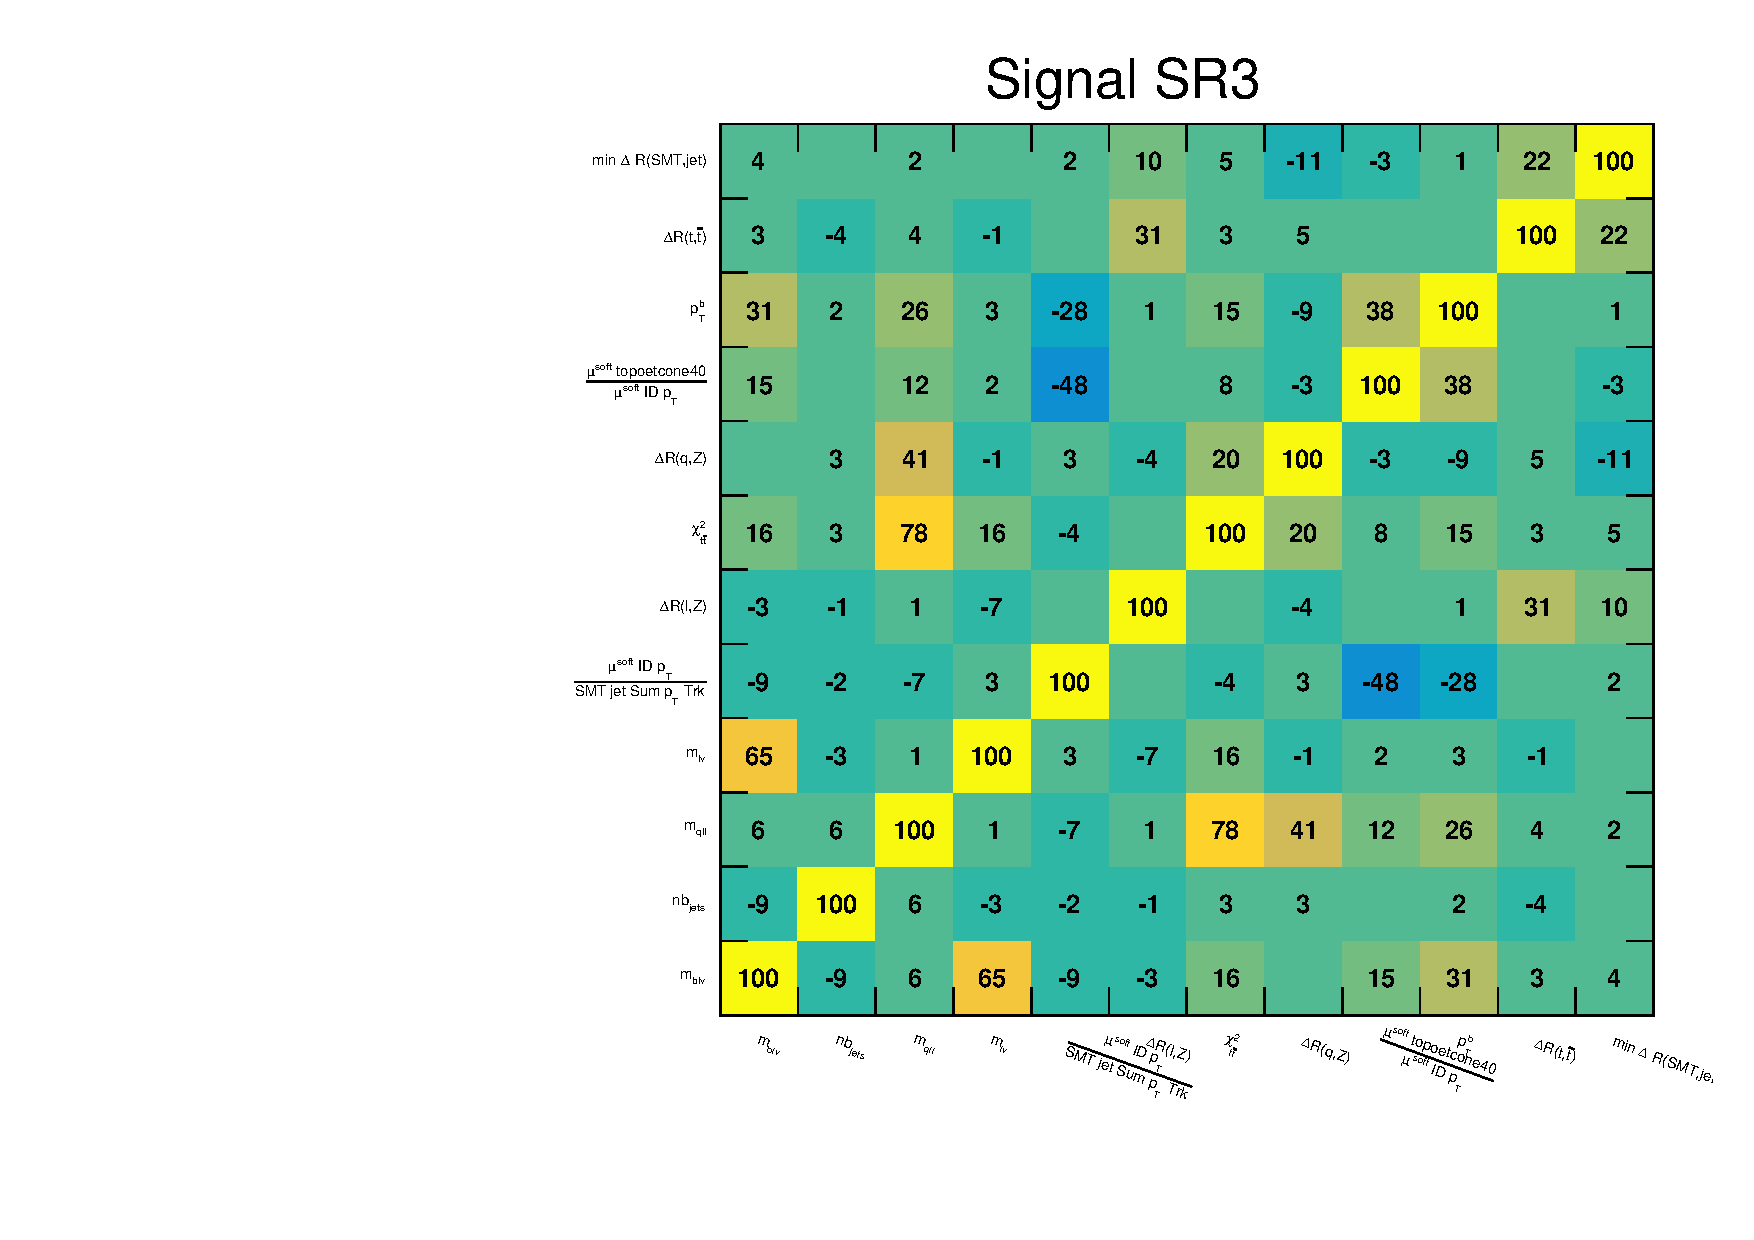
\includegraphics[width=.7\textwidth]{Chapters/CH6/figures/SR3_UsingSMT/BDT/RedSet/CorrMatrix_sig}\\
		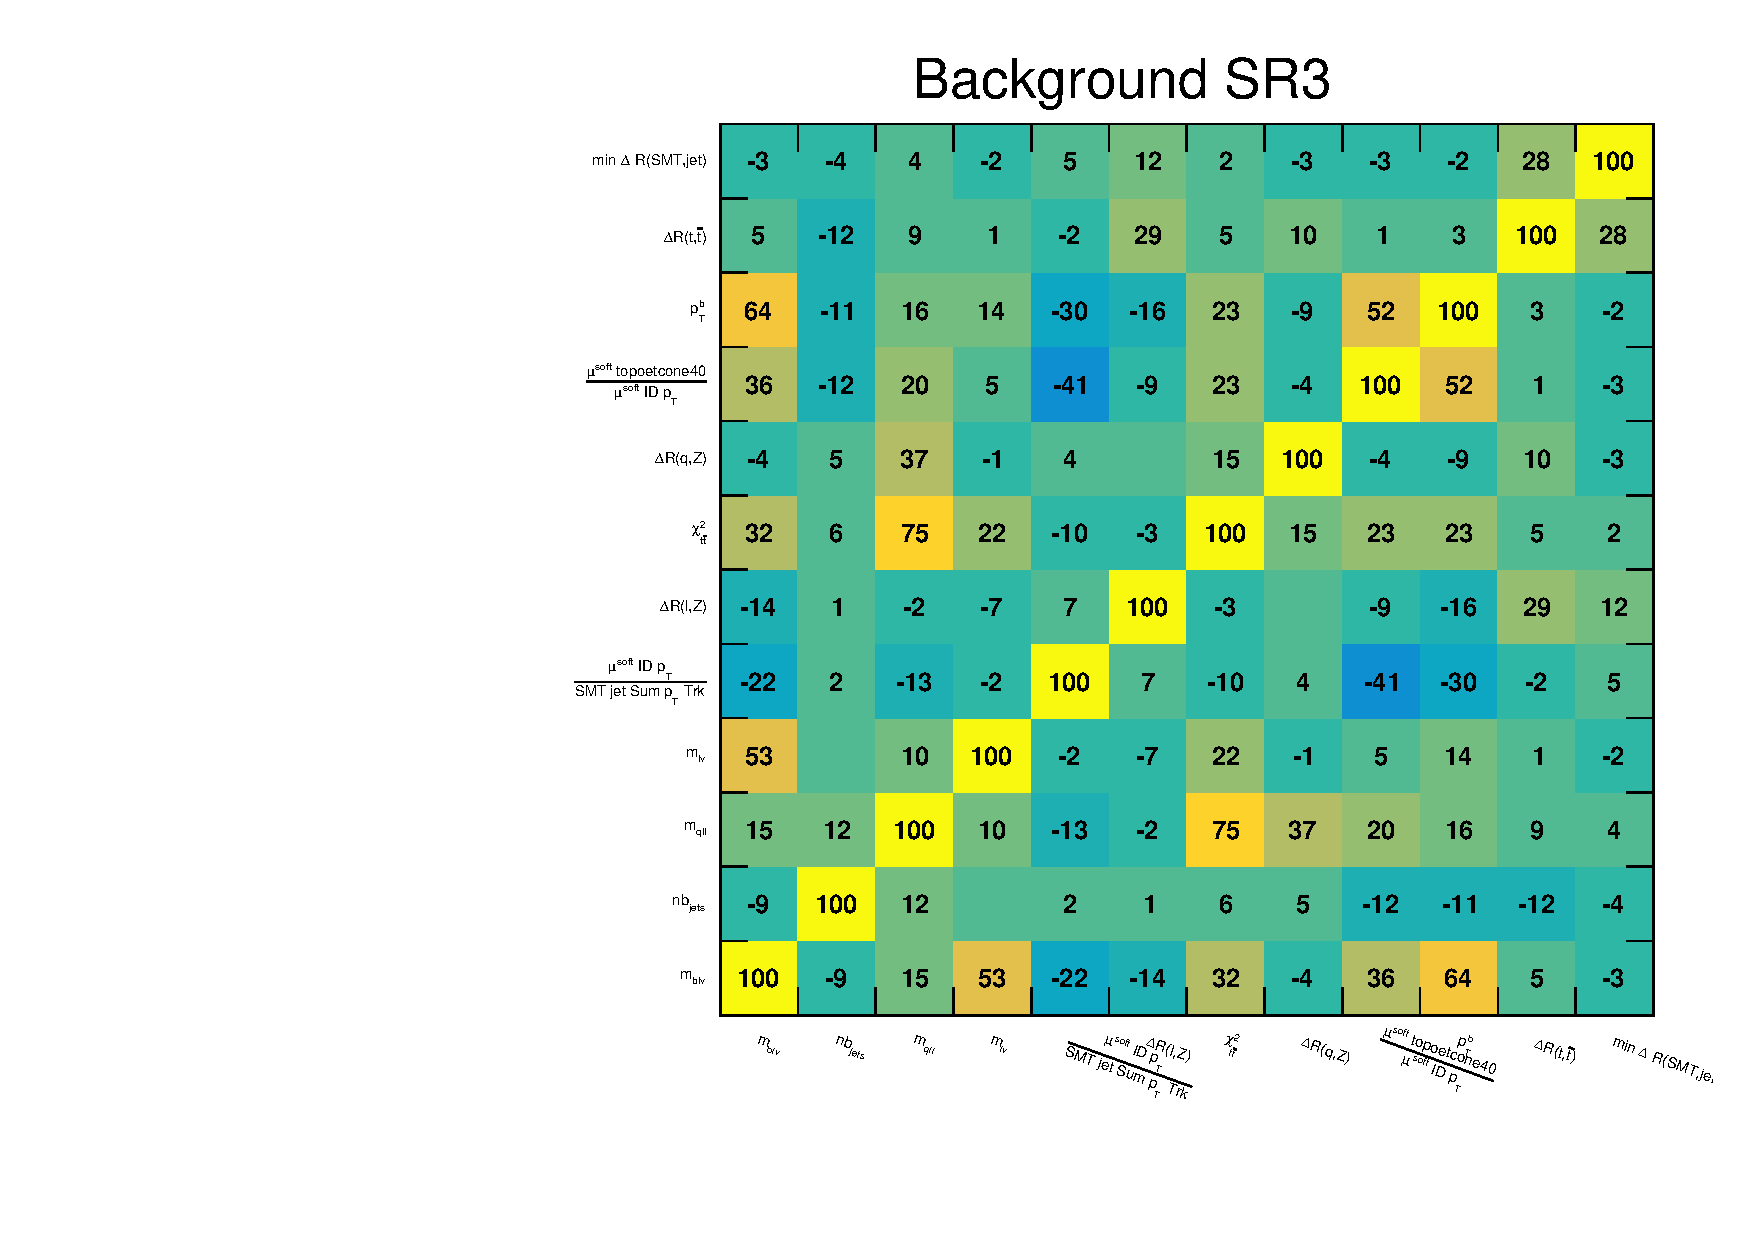
\includegraphics[width=.7\textwidth]{Chapters/CH6/figures/SR3_UsingSMT/BDT/RedSet/CorrMatrix_bkg}
	\end{tabular}
	\caption{ Correlation matrix of the input variables from signal (top) and background (bottom) samples
		considered in the training of the GBDT in SR3 to built the \Dthree discriminant for \tZc coupling search.}
	\label{app:BDT:fig:D3inputCorrMatrix}
\end{figure}

\begin{table}[!htbp]
	\scriptsize
	\centering
	%\documentclass[a4paper]{article}
%\usepackage[T1]{fontenc}
%\usepackage[utf8]{inputenc}
%\usepackage{booktabs}
%\begin{document}
\begin{tabular}{ccc}
\toprule
Variable & $\langle s^{2}\rangle$  & Definition \\
\midrule
$m_{b\ell\nu}$  &  0.1717  &  SM top-quark candidate mass  \\
$N\,b\,jets$  &  0.08218  &  Number of b-jets tagged with DL1r  \\
$m_{q\ell\ell}$  &  0.07019  &  FCNC top-quark candidate mass  \\
$\frac{\mu^{soft} ID p_{T}}{SMT\,jet\,Sum p_{T} Trk}$  &  0.03357  &  Ratio between the soft muon ID pT and pT sum of tracks  \\
$\Delta R(\ell,Z)$  &  0.03141  &  $\Delta R$ between $W$ boson lepton and $Z$ boson candidates  \\
$\Delta R(t_{\text{SM}},t_{\text{FCNC}})$  &  0.02508  &  $\Delta R$ between SM and FCNC top-quark candidates  \\
$\Delta R(\mu^{soft},Z)$  &  0.006596  &  $\Delta R$ between soft muon and $Z$ boson candidates  \\
\bottomrule
\end{tabular}
%\end{document}

	\caption{
		Final set of input variables considered in the training of the GBDT in SR3 to built the \Dthree discriminant.
		Variables are ordered by the separation $\langle s^{2}\rangle$ value.
	}%
	\label{app:BDT:tab:D3inputFinalSet}
\end{table}



\begin{figure}[!h]
	\centering
	\begin{tabular}{ccc}
		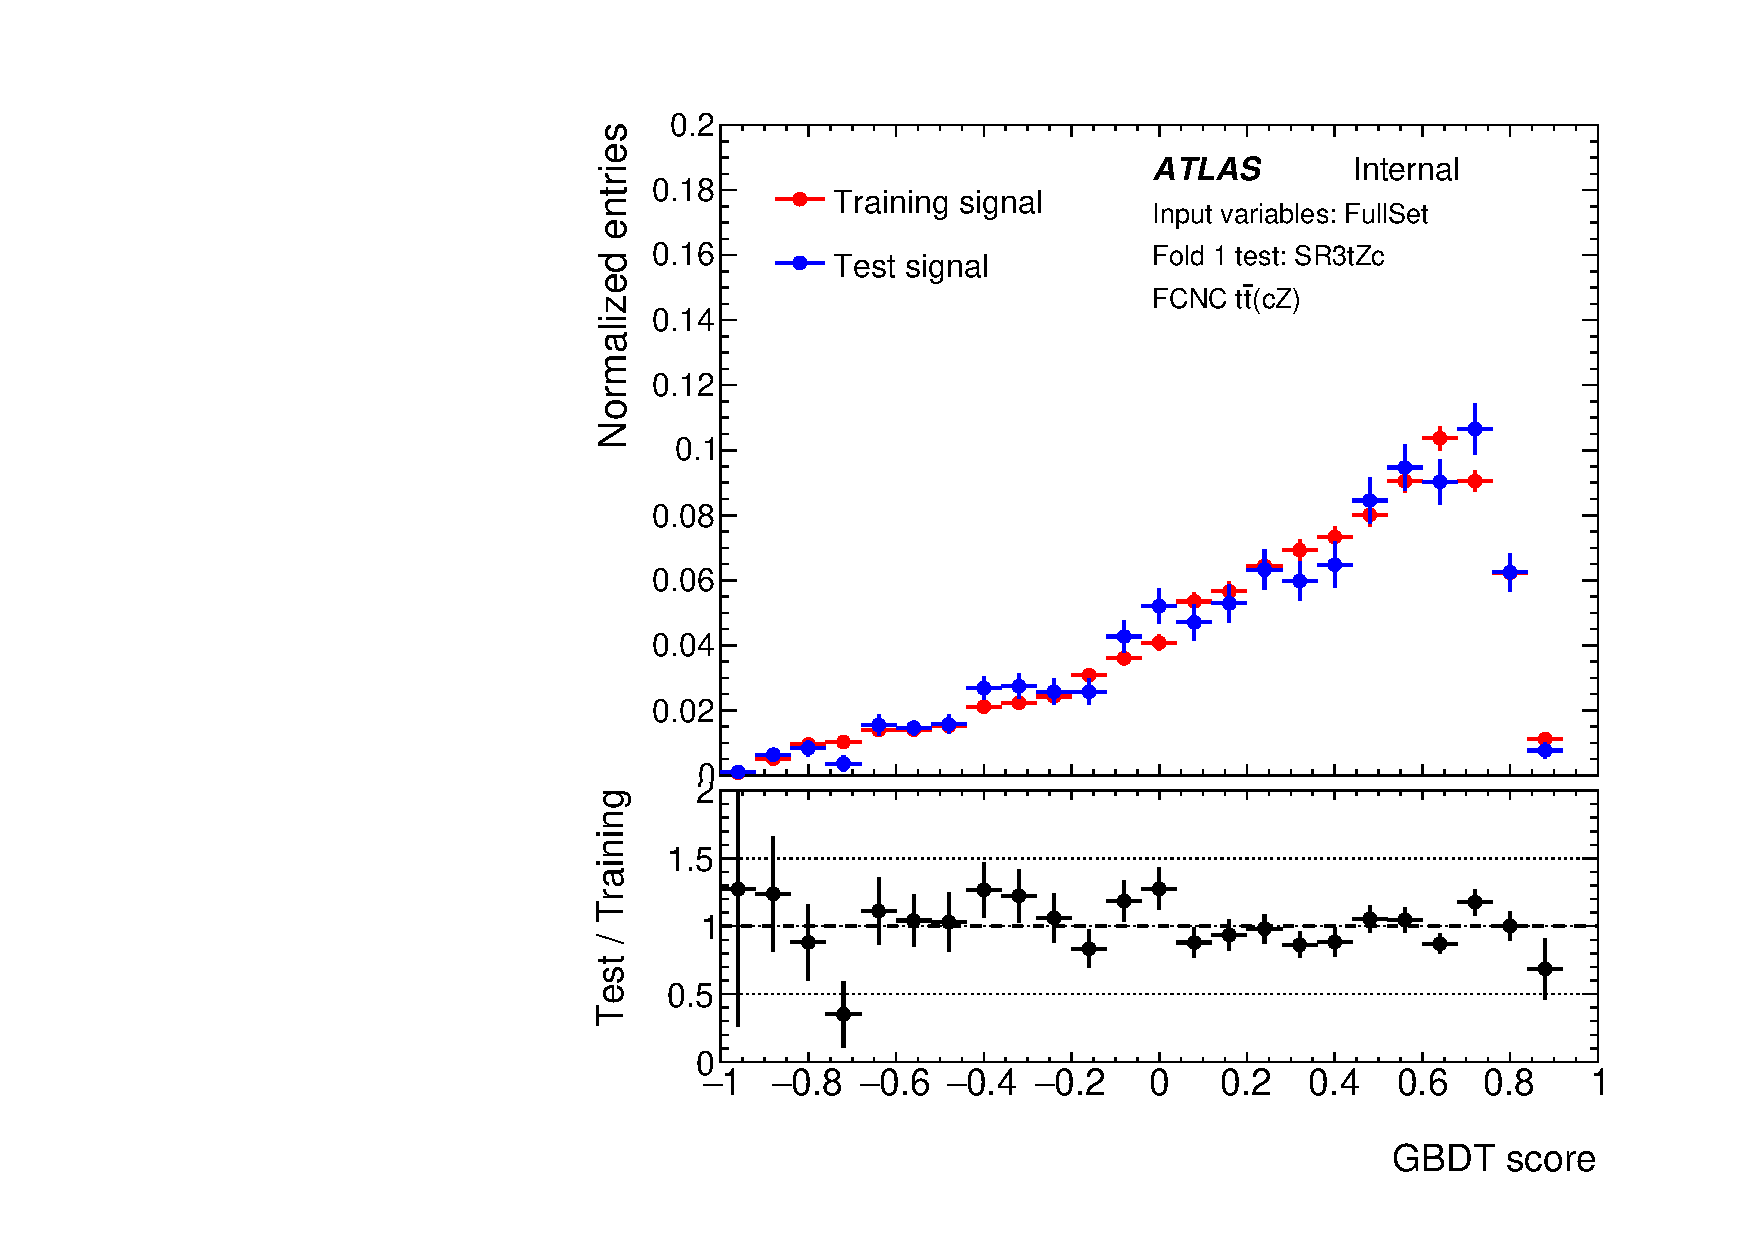
\includegraphics[width=.30\textwidth]{Chapters/CH6/figures/SR3_UsingSMT/BDT/RedSet/GBDT_signal_FullSet_Fold1} &
		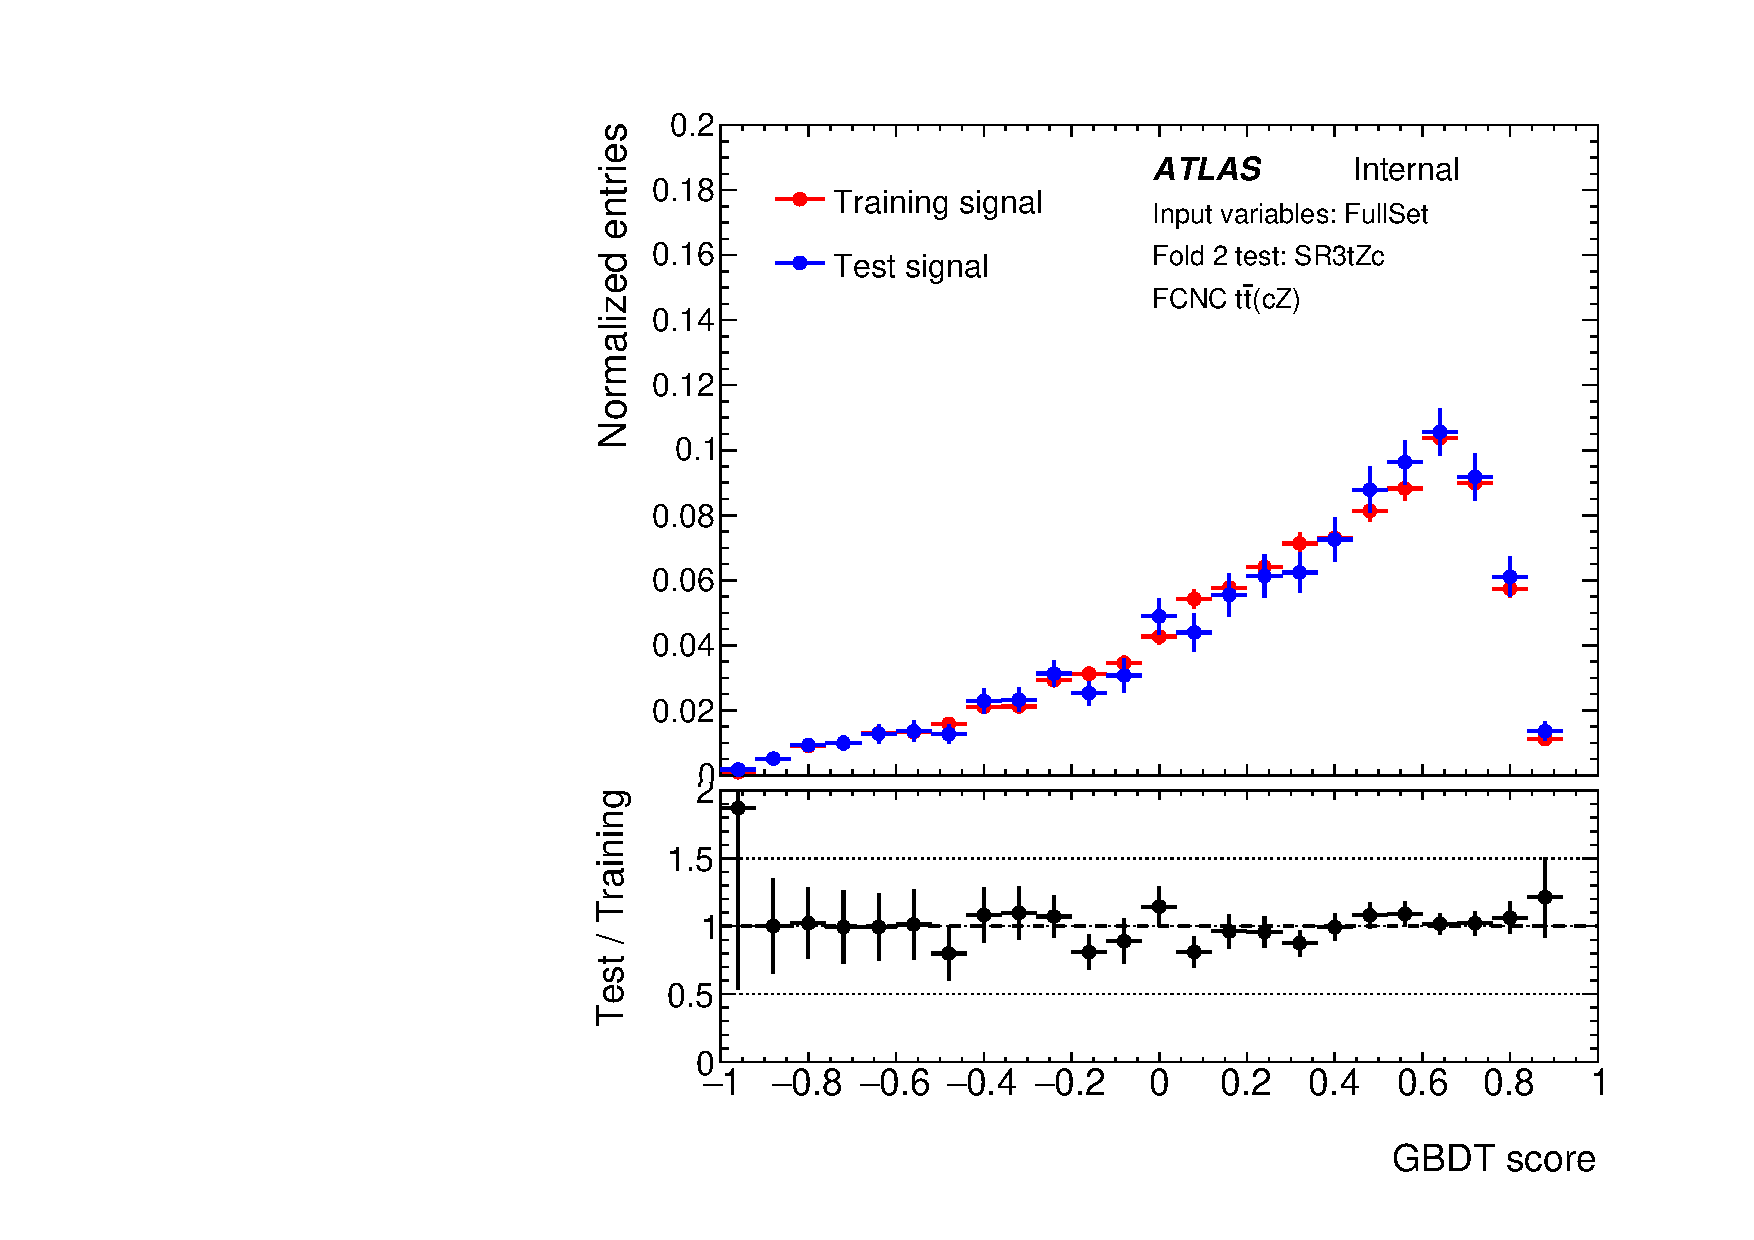
\includegraphics[width=.30\textwidth]{Chapters/CH6/figures/SR3_UsingSMT/BDT/RedSet/GBDT_signal_FullSet_Fold2} &
		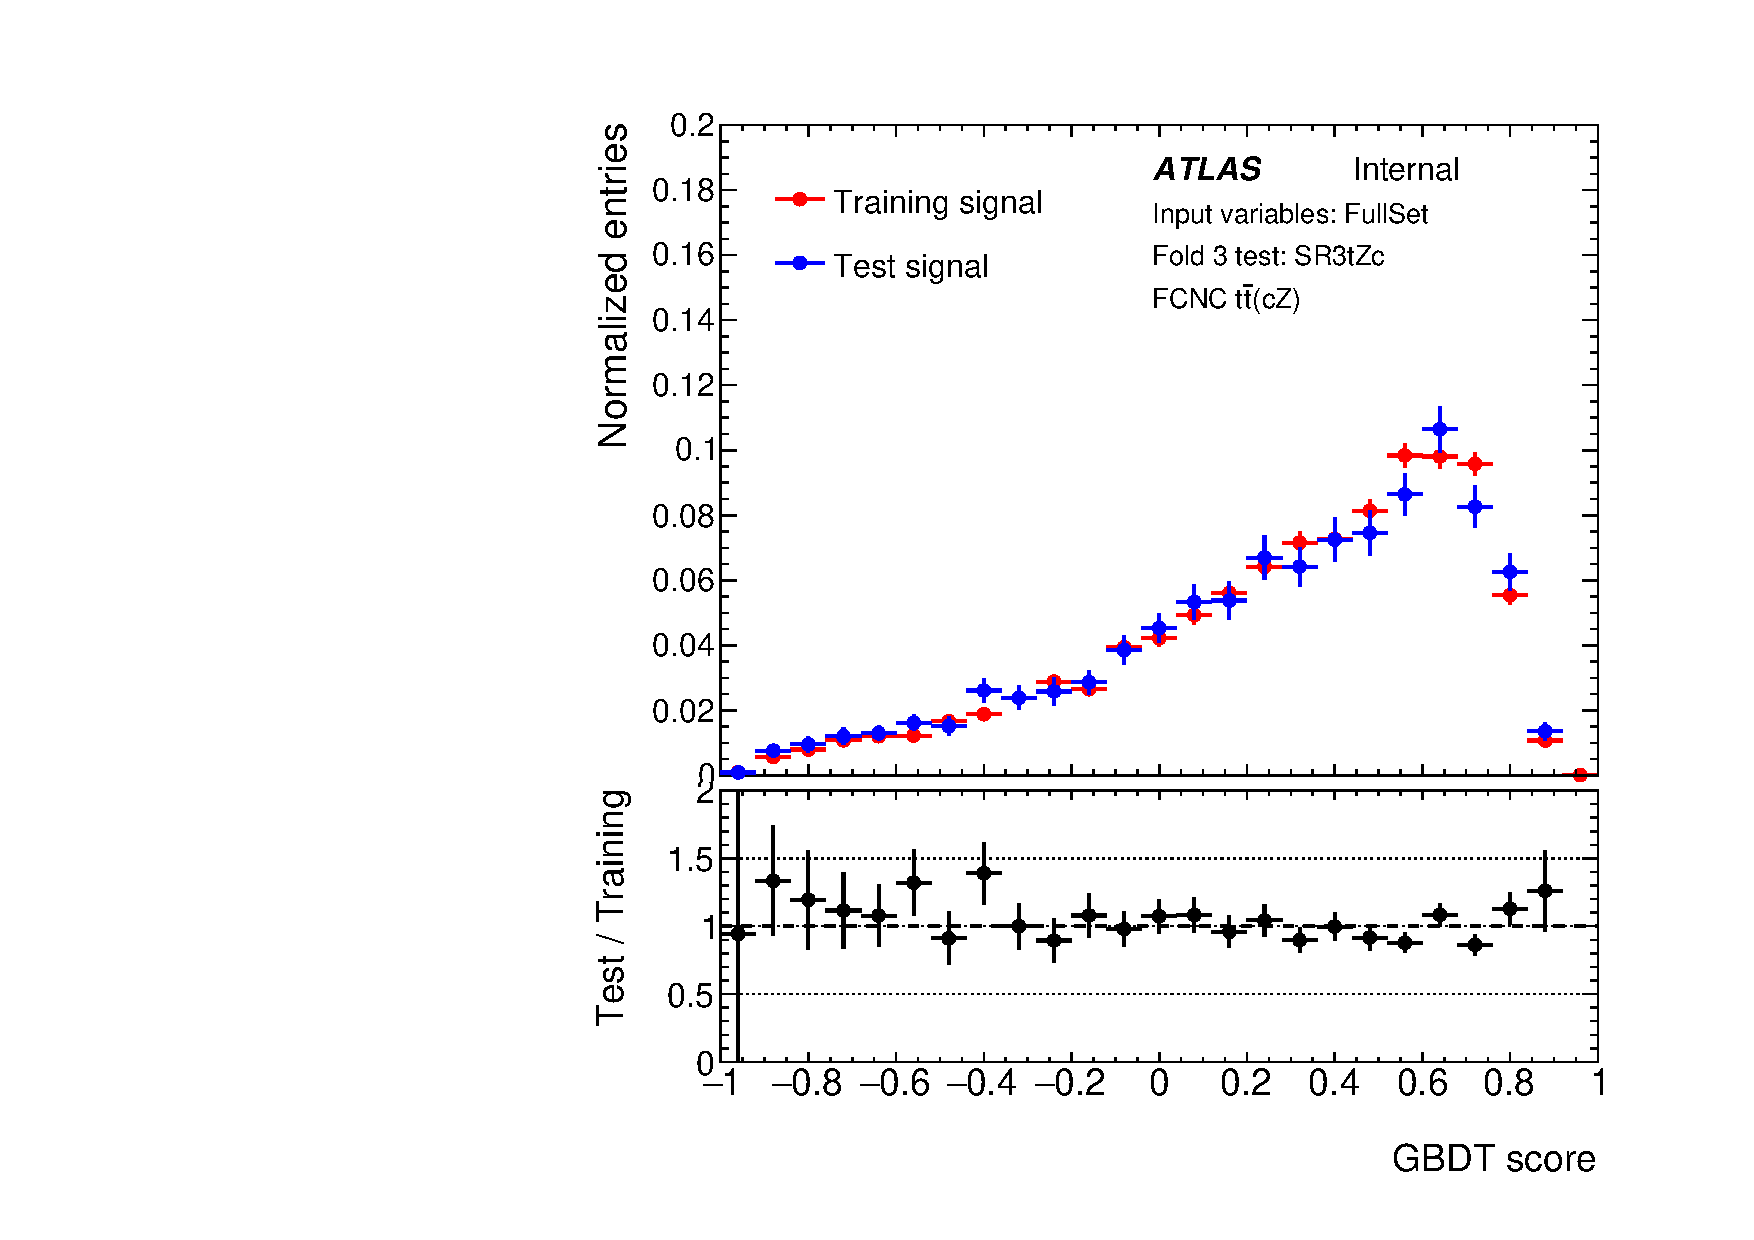
\includegraphics[width=.30\textwidth]{Chapters/CH6/figures/SR3_UsingSMT/BDT/RedSet/GBDT_signal_FullSet_Fold3} \\
		\multicolumn{3}{c}{
			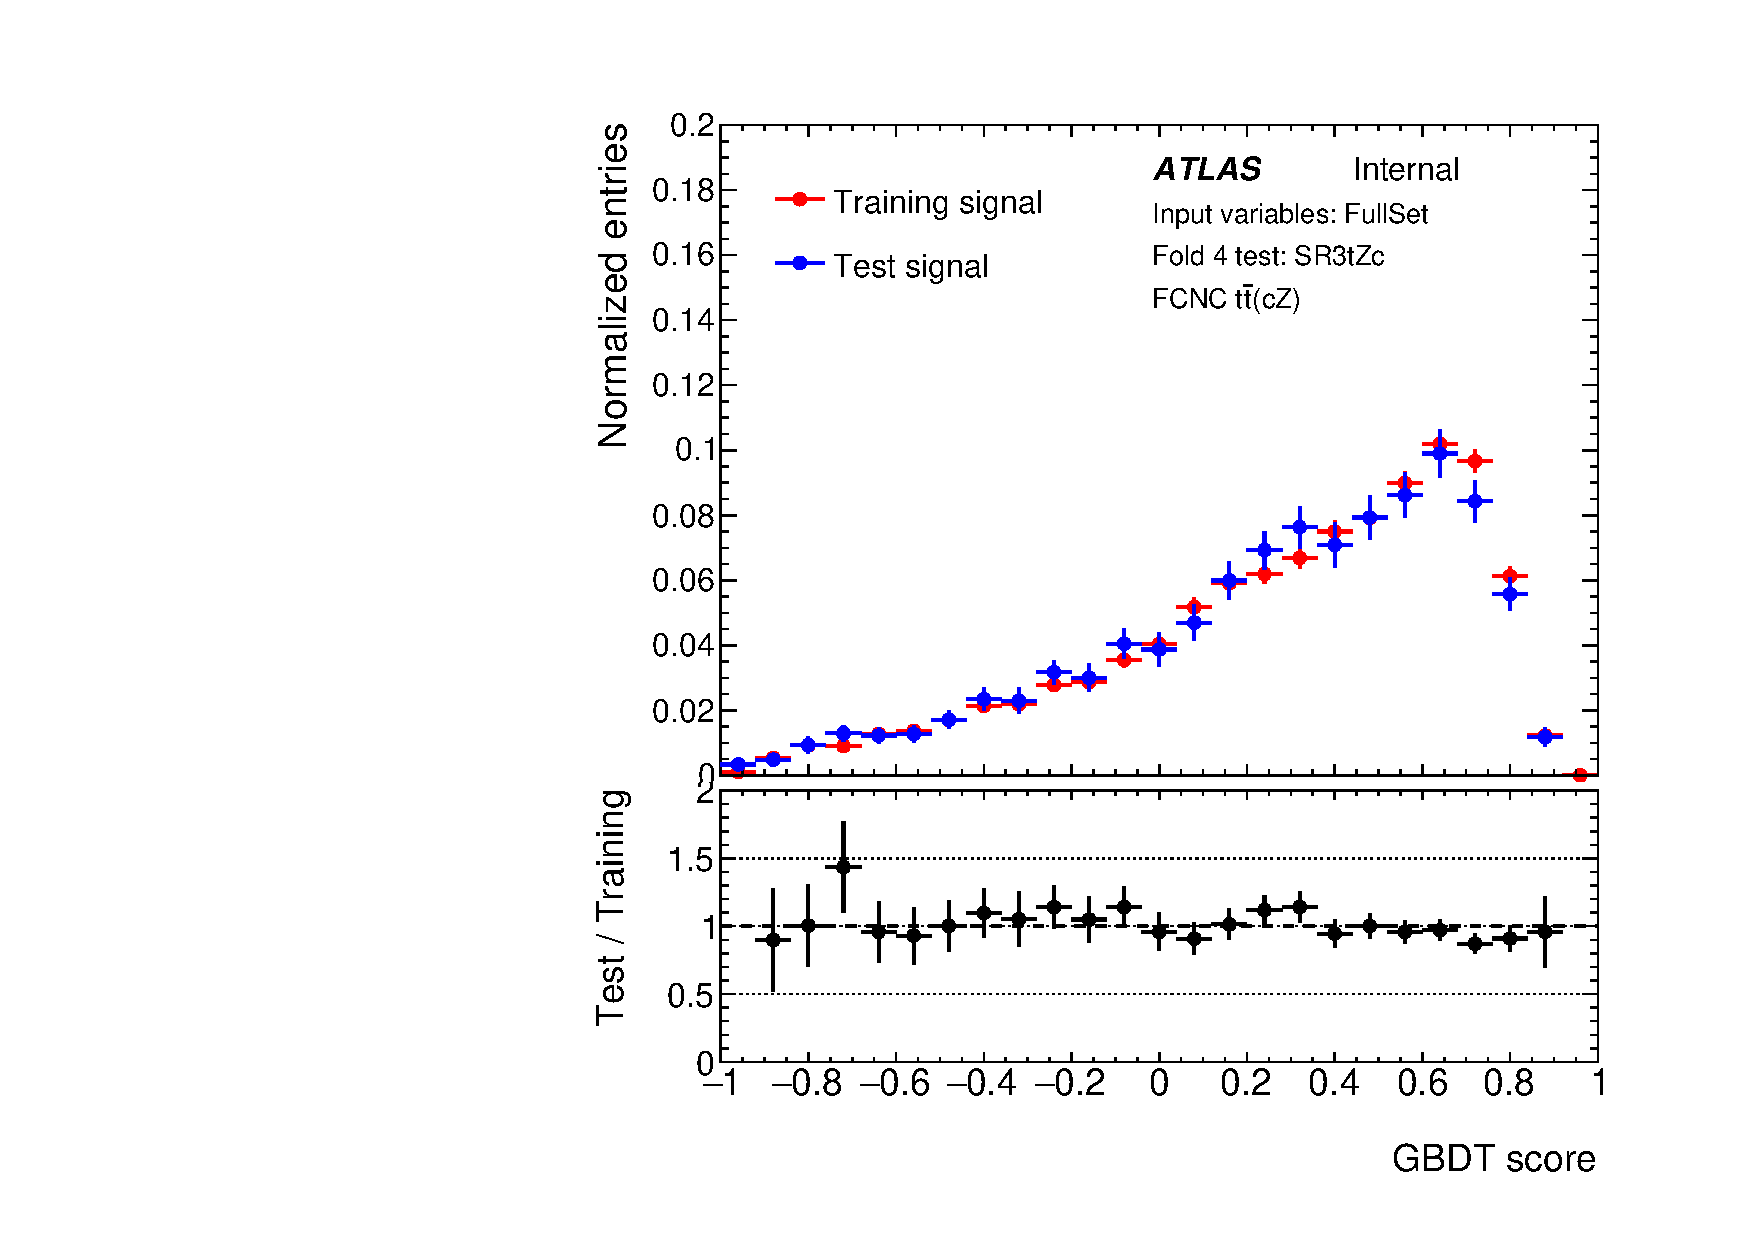
\includegraphics[width=.30\textwidth]{Chapters/CH6/figures/SR3_UsingSMT/BDT/RedSet/GBDT_signal_FullSet_Fold4}
			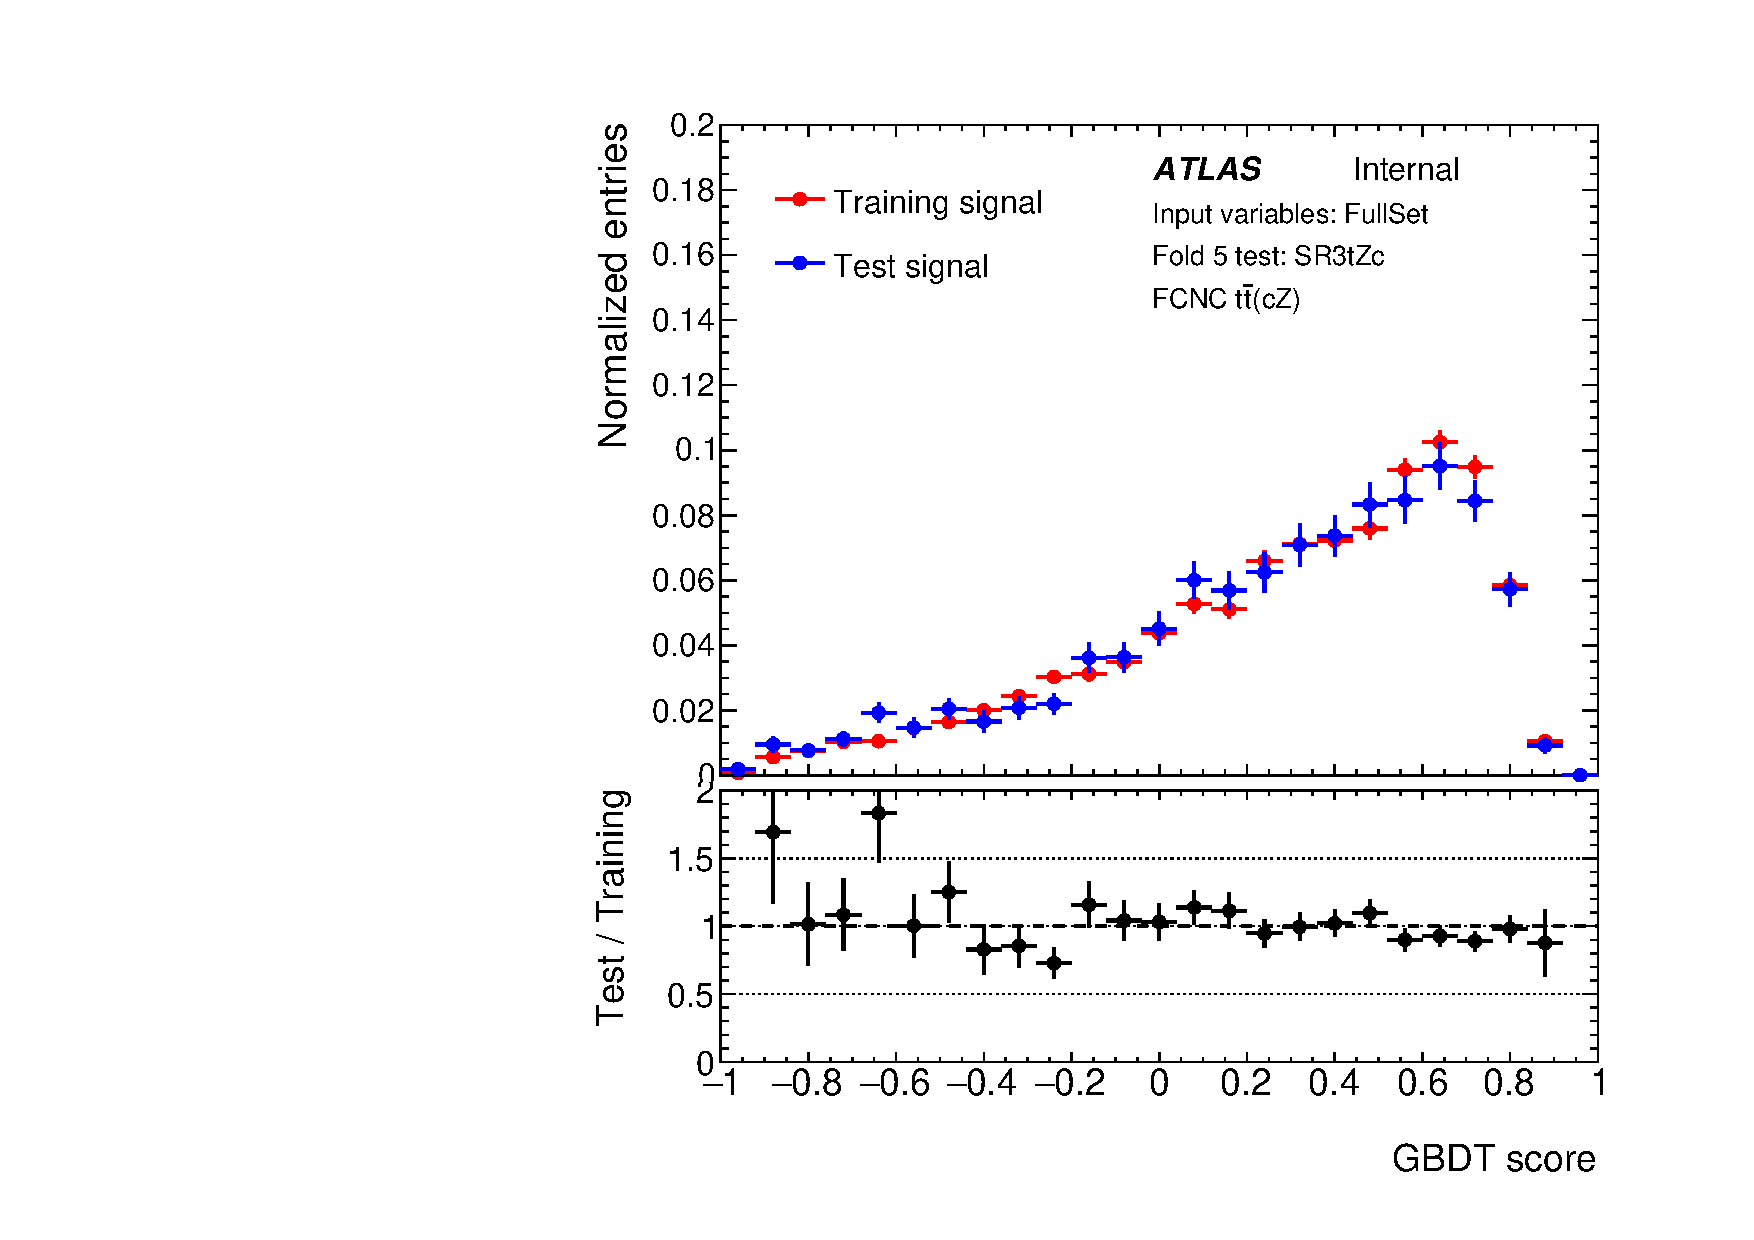
\includegraphics[width=.30\textwidth]{Chapters/CH6/figures/SR3_UsingSMT/BDT/RedSet/GBDT_signal_FullSet_Fold5}} \\
	\end{tabular}
	\caption{ The FCNC \ttbar decay signal GBDT output score distribution for each of five GBDTs trained in SR3 for the \Dthree discriminant.
		Initial (full) set of input variables is used in the training.
		Comparing results between training and test samples.
	}%
	\label{app:BDT:fig:SR3:GBDTsigFullSet}
\end{figure}
\begin{figure}[!h]
	\centering
	\begin{tabular}{ccc}
		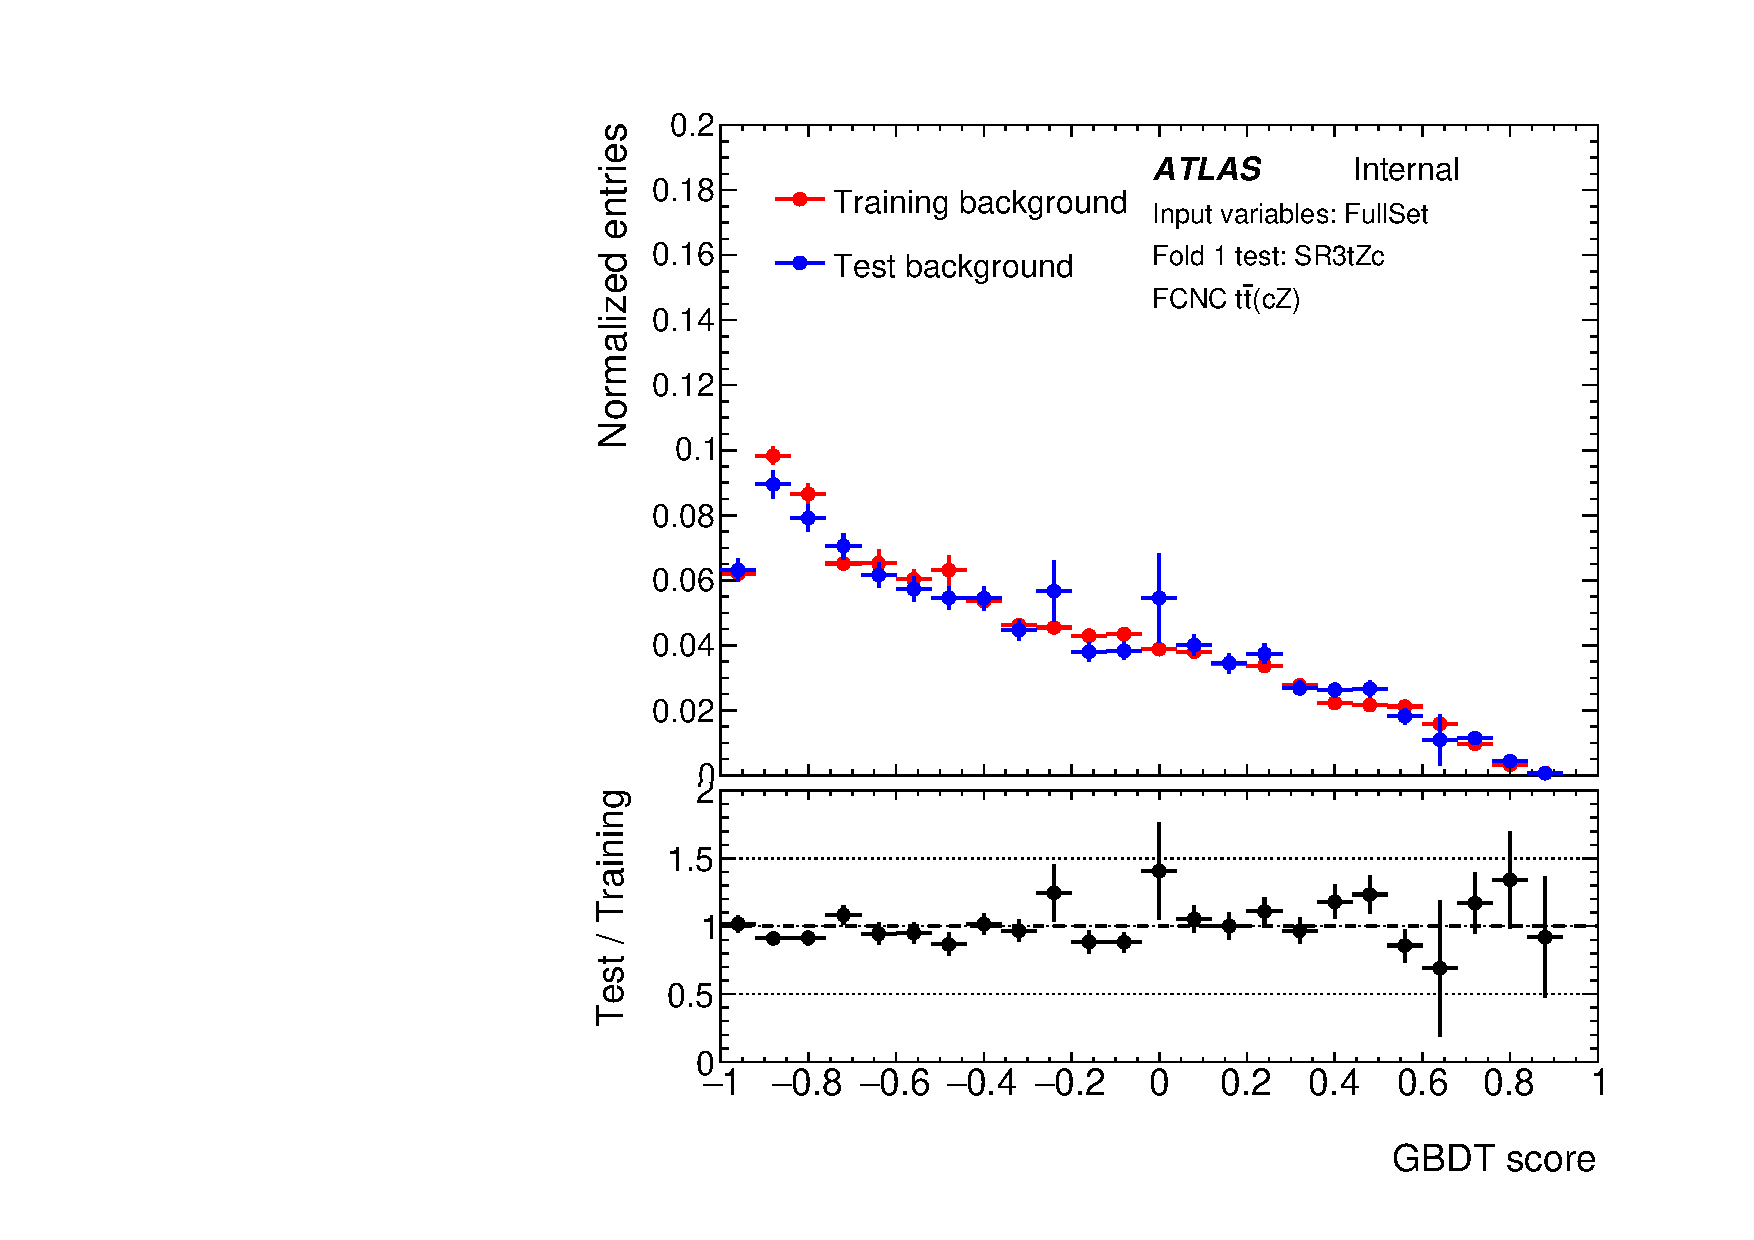
\includegraphics[width=.295\textwidth]{Chapters/CH6/figures/SR3_UsingSMT/BDT/RedSet/GBDT_background_FullSet_Fold1} &
		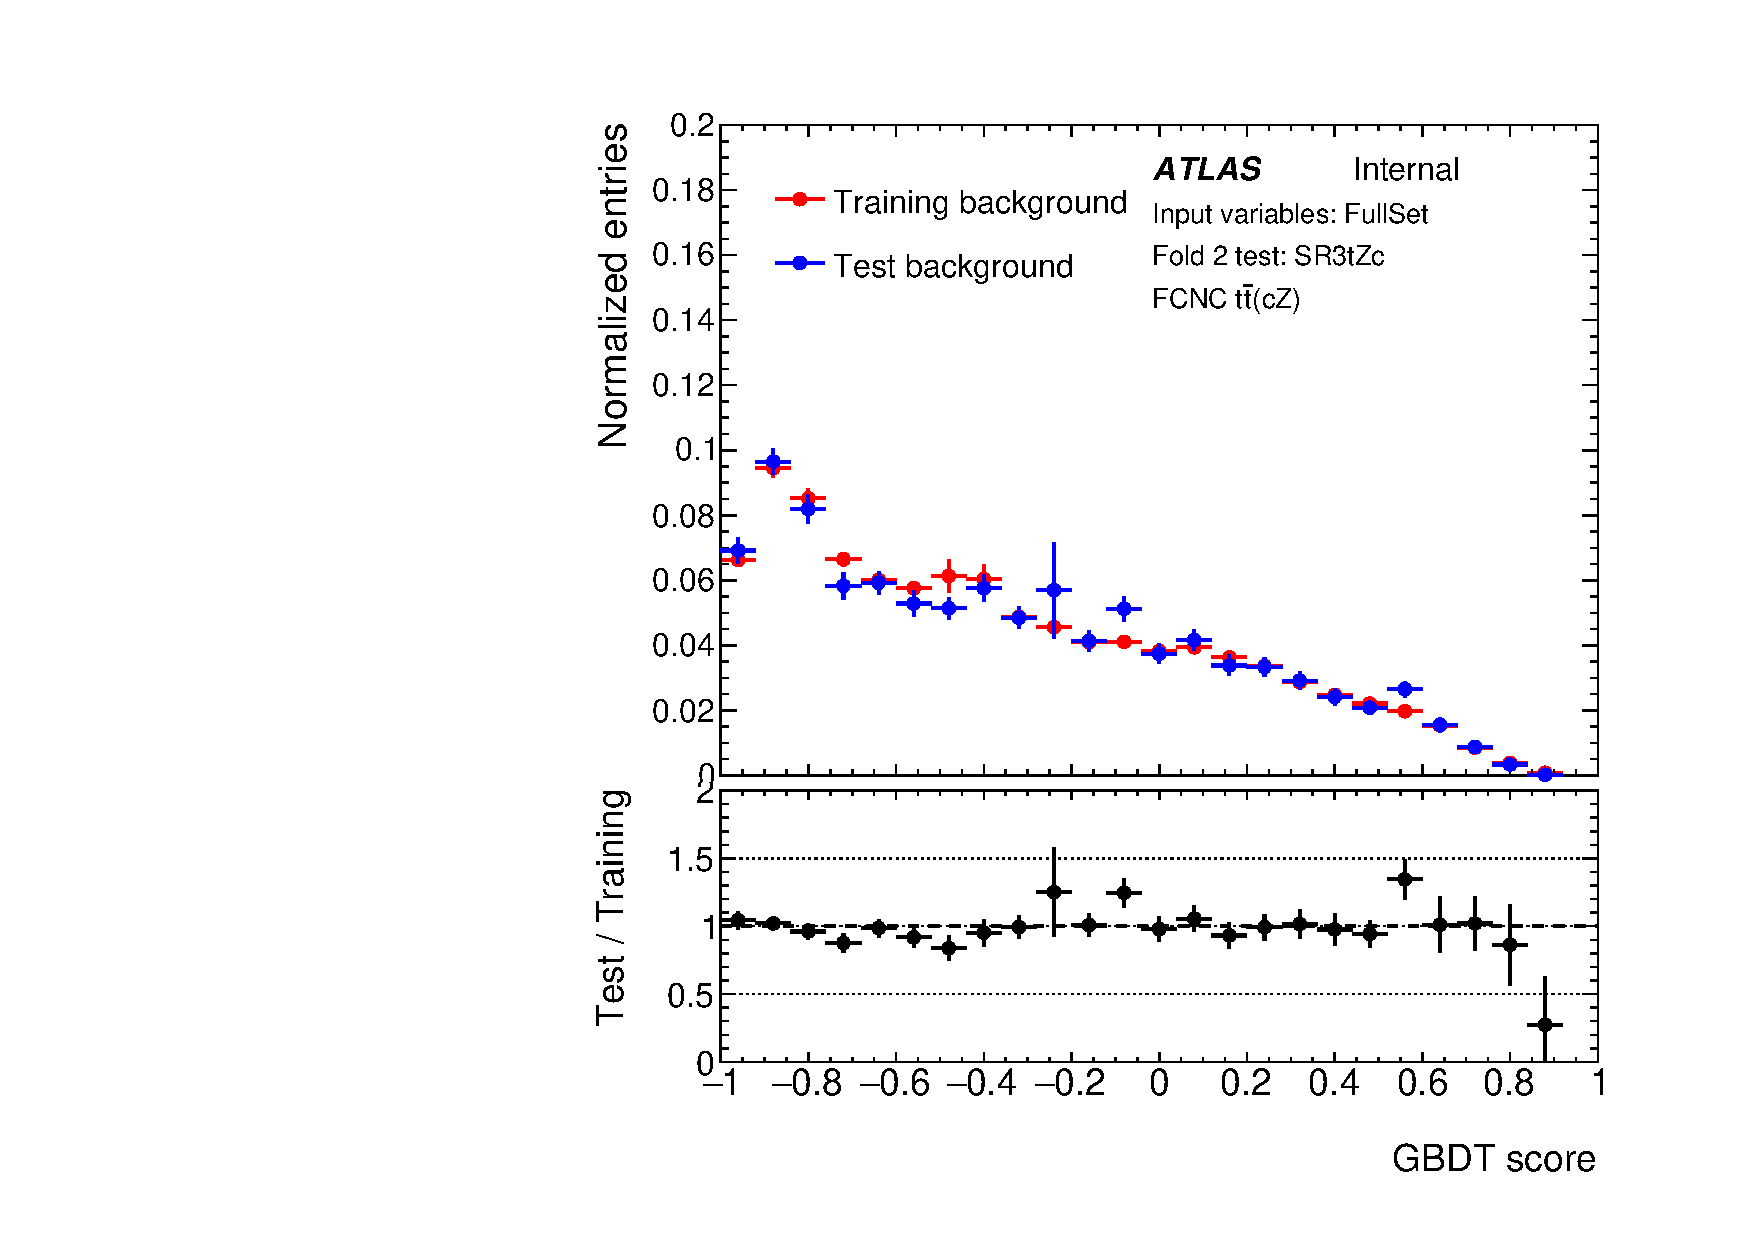
\includegraphics[width=.295\textwidth]{Chapters/CH6/figures/SR3_UsingSMT/BDT/RedSet/GBDT_background_FullSet_Fold2} &
		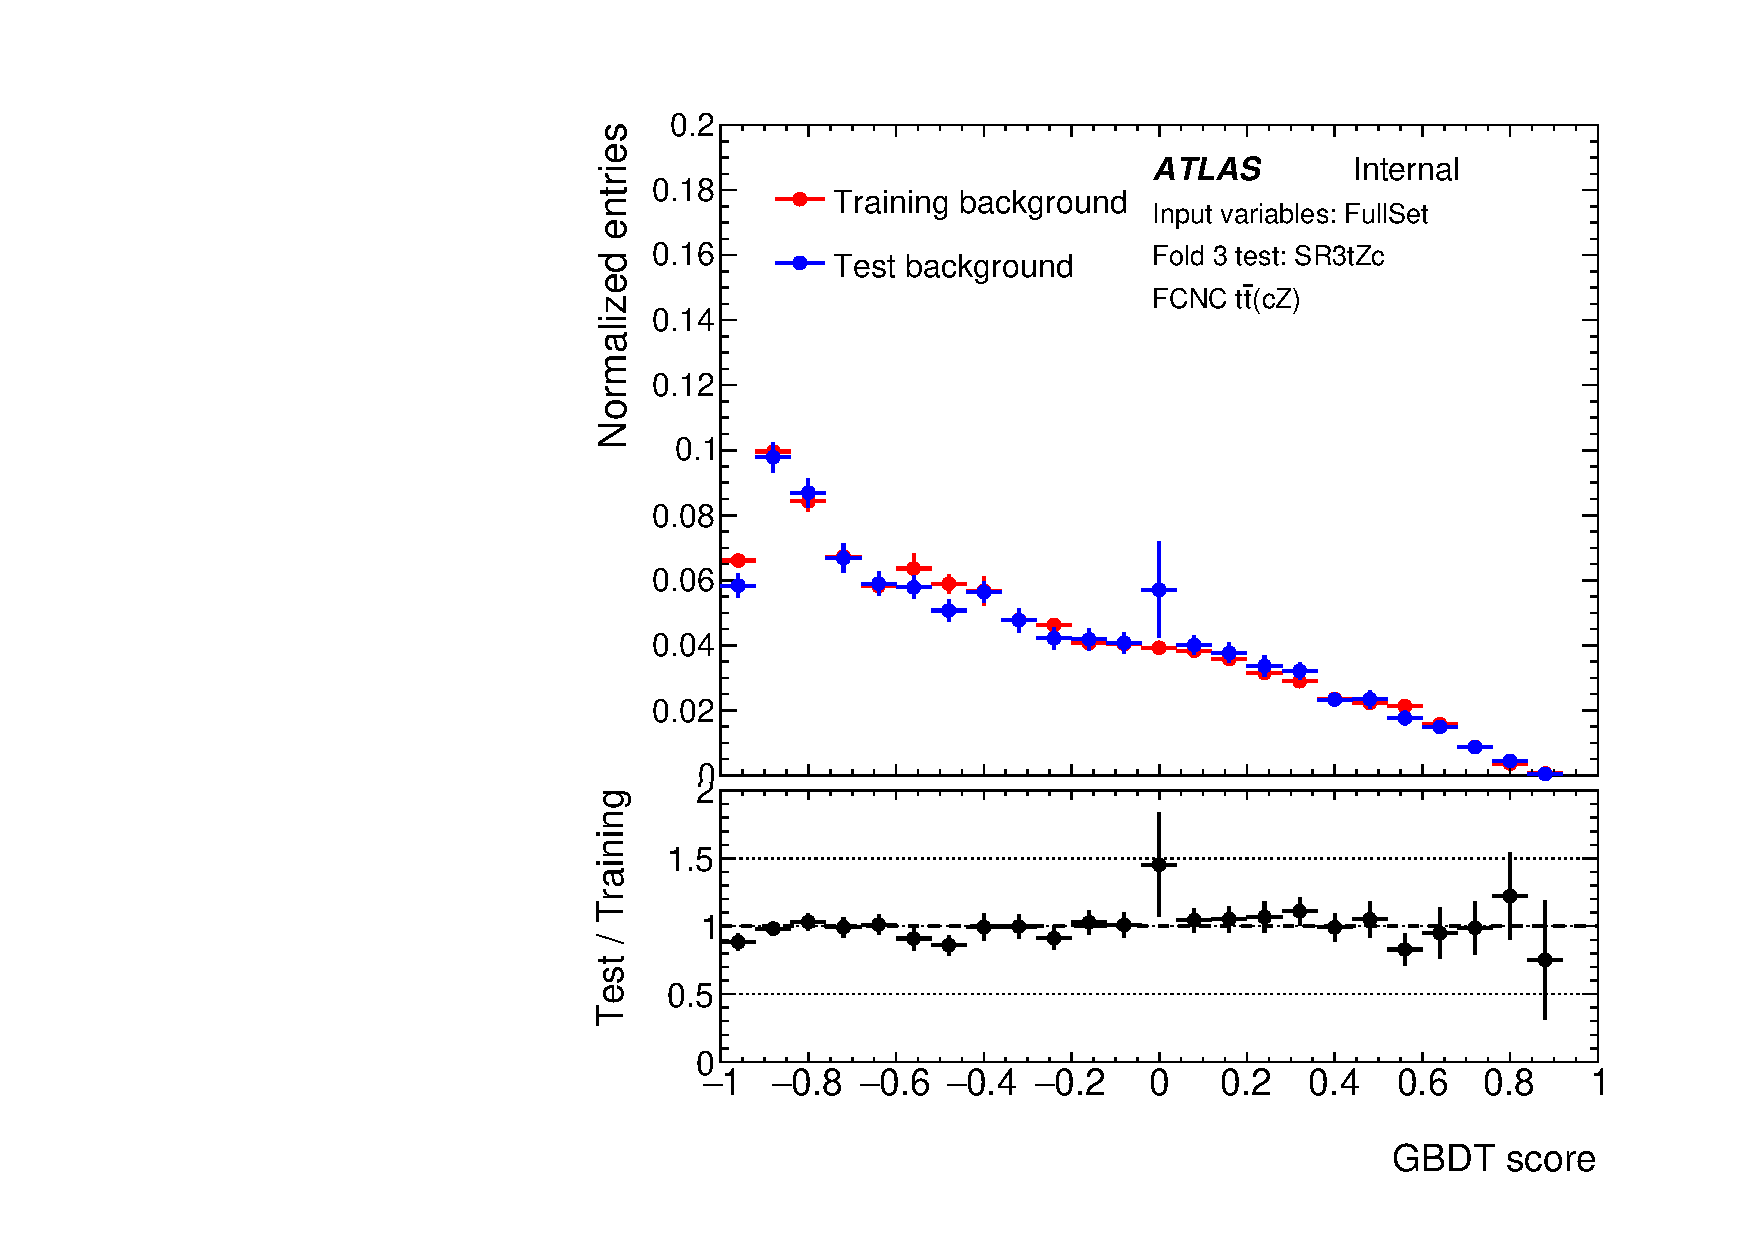
\includegraphics[width=.295\textwidth]{Chapters/CH6/figures/SR3_UsingSMT/BDT/RedSet/GBDT_background_FullSet_Fold3} \\
		\multicolumn{3}{c}{
			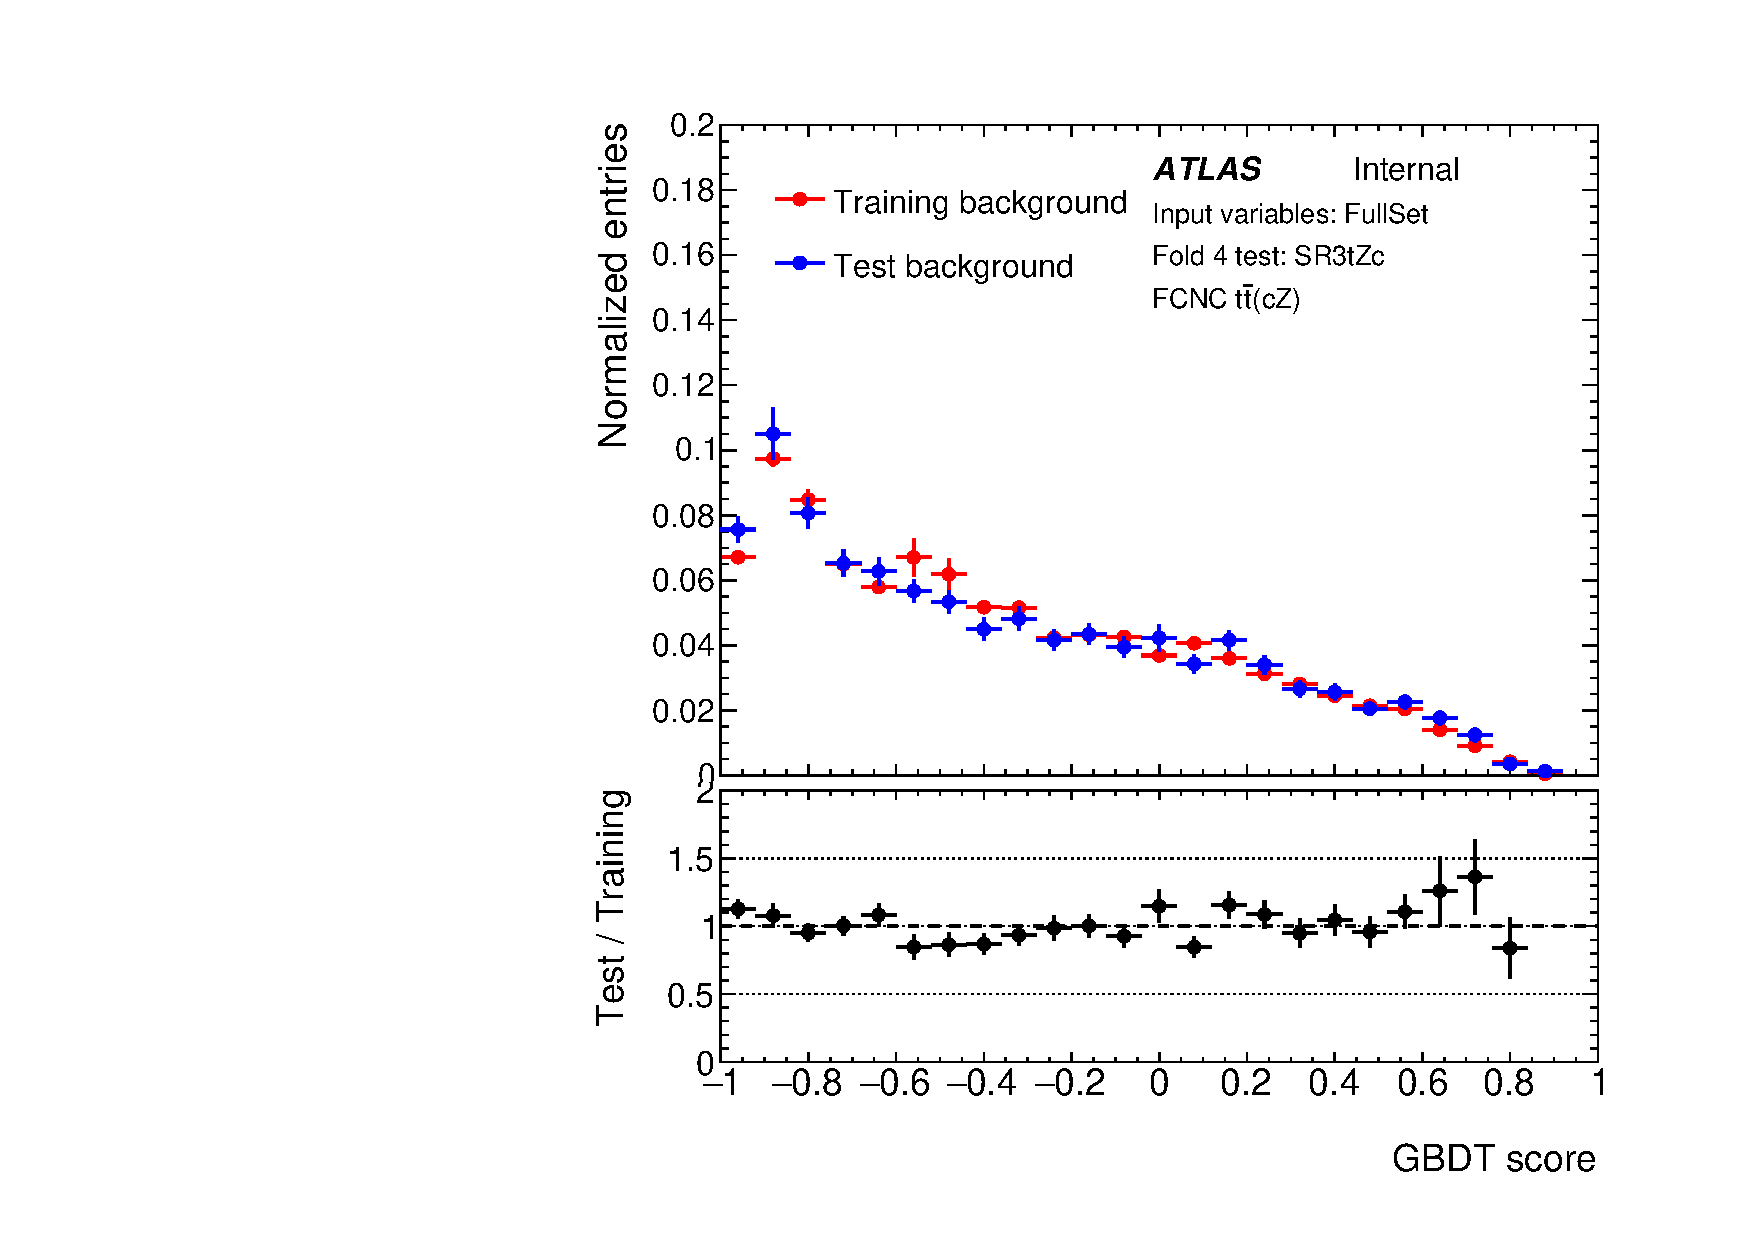
\includegraphics[width=.295\textwidth]{Chapters/CH6/figures/SR3_UsingSMT/BDT/RedSet/GBDT_background_FullSet_Fold4}
			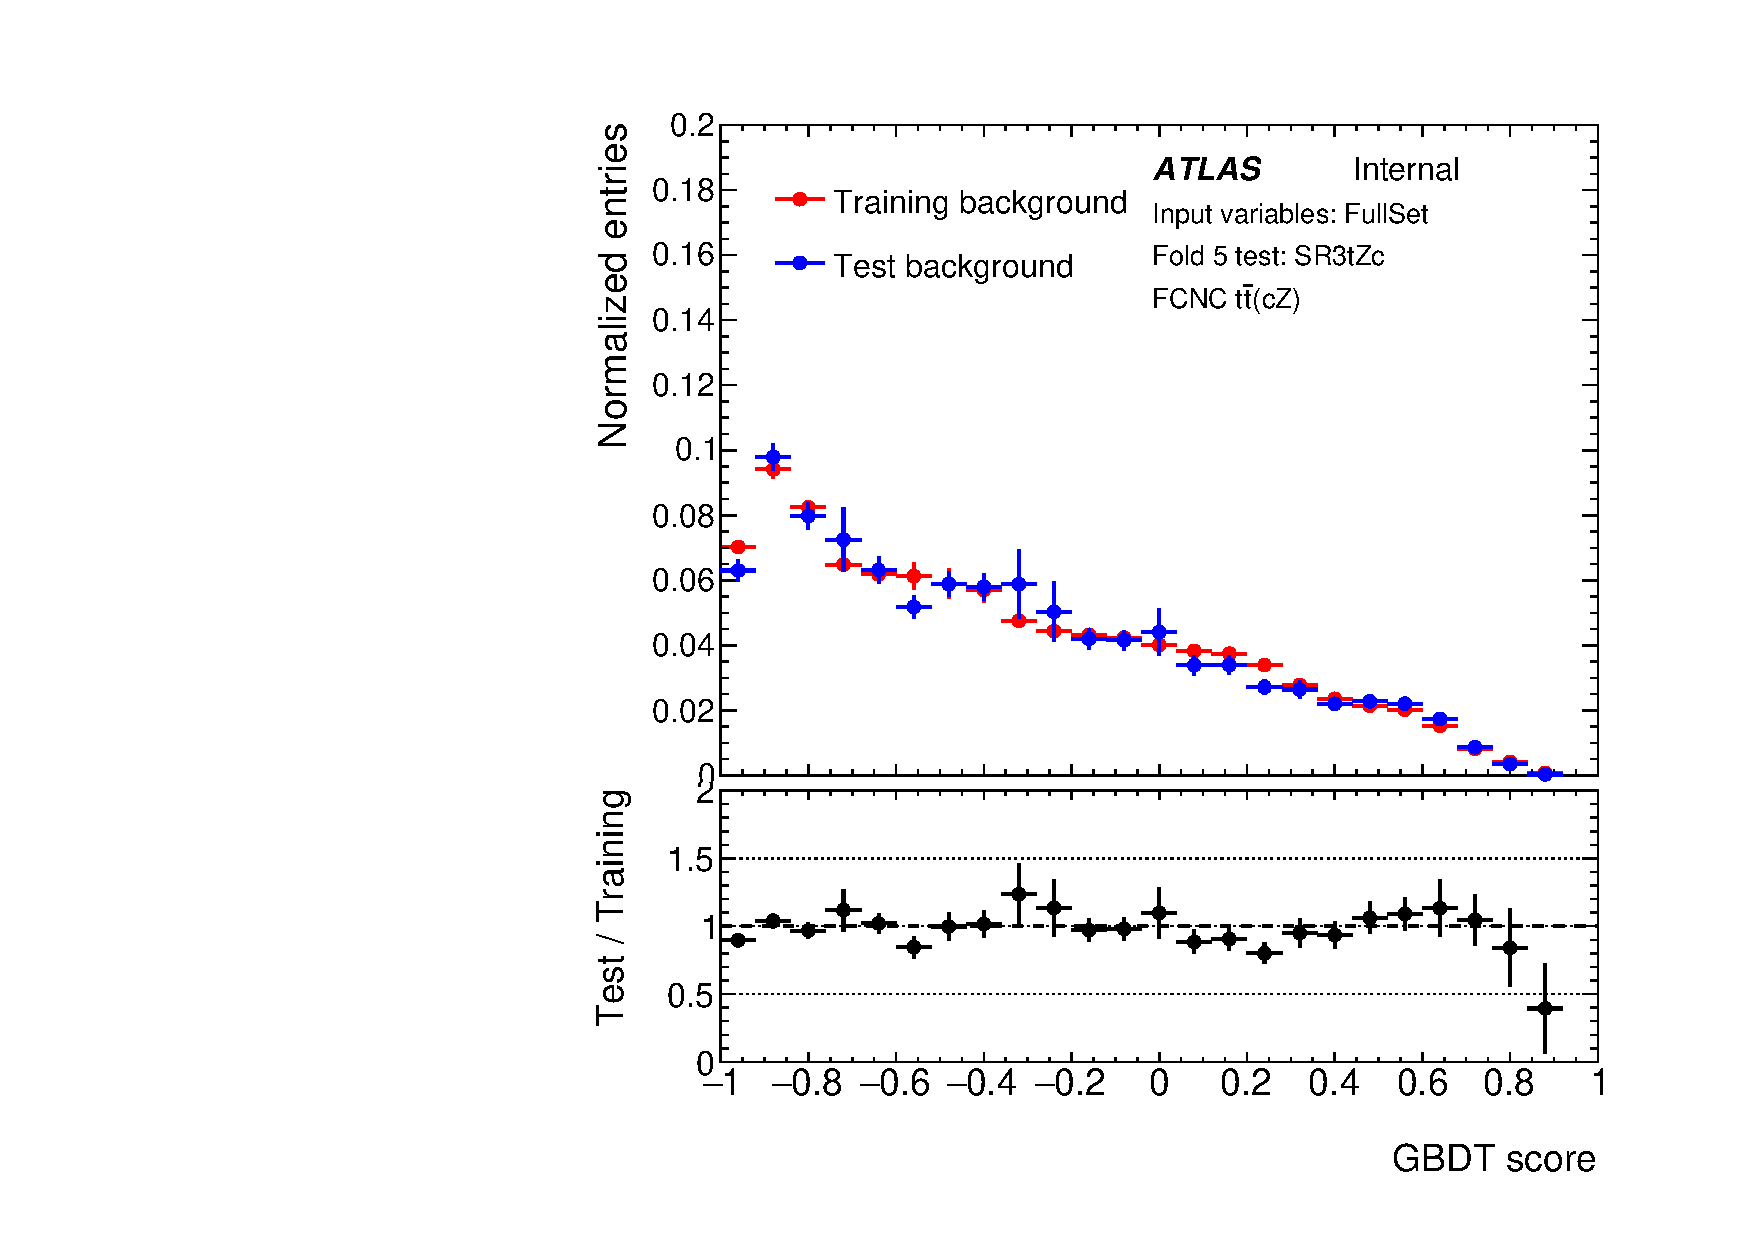
\includegraphics[width=.295\textwidth]{Chapters/CH6/figures/SR3_UsingSMT/BDT/RedSet/GBDT_background_FullSet_Fold5}} \\
	\end{tabular}
	\caption{ The background GBDT output score distribution for each of five GBDTs trained in SR3 for the \Dthree discriminant.
		Initial (full) set of input variables is used in the training.
		Comparing results between training and test samples.
	}%
	\label{app:BDT:fig:SR3:GBDTbkgFullSet}
\end{figure}


\begin{figure}[!htbp]
	\centering
	\begin{tabular}{ccc}
		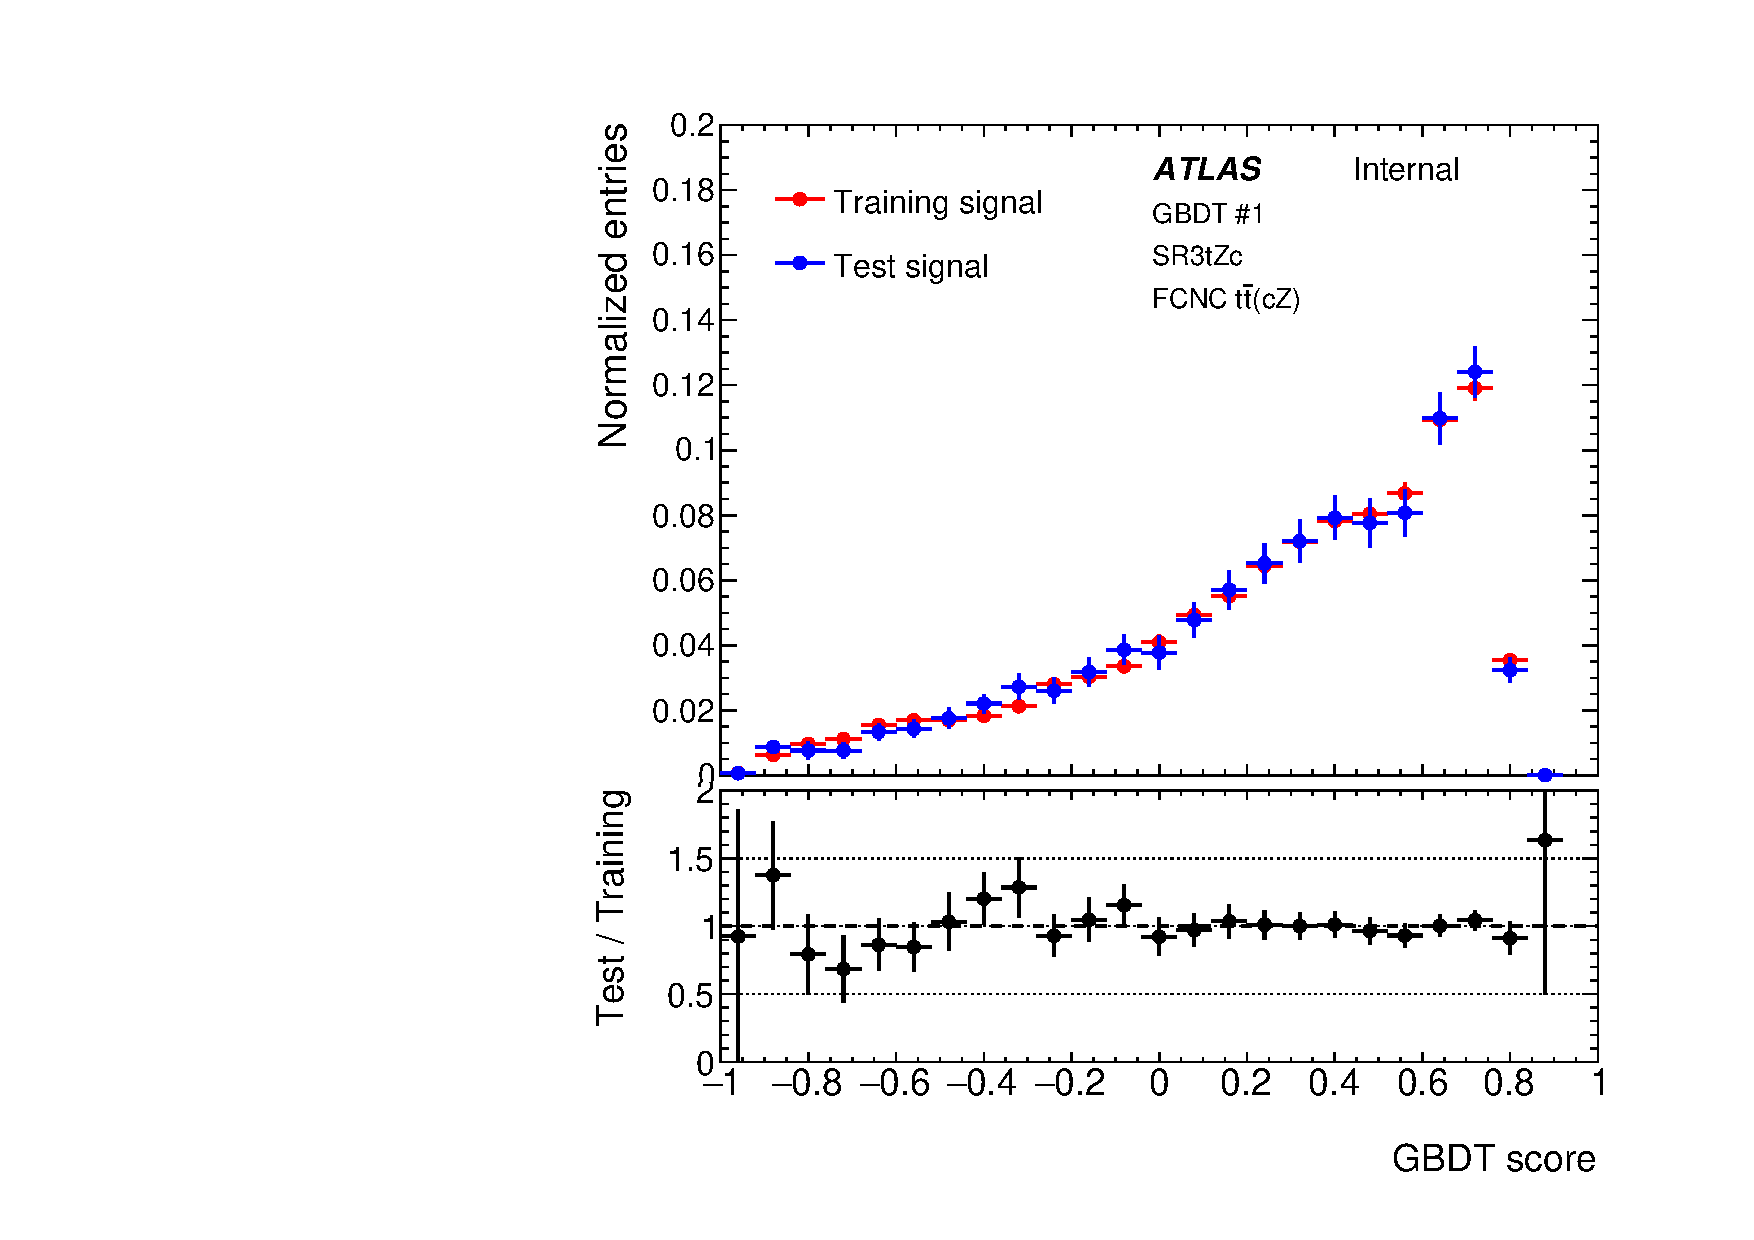
\includegraphics[width=.3\textwidth]{Chapters/CH6/figures/SR3_UsingSMT/BDT/GBDT_signal_Fold1} &
		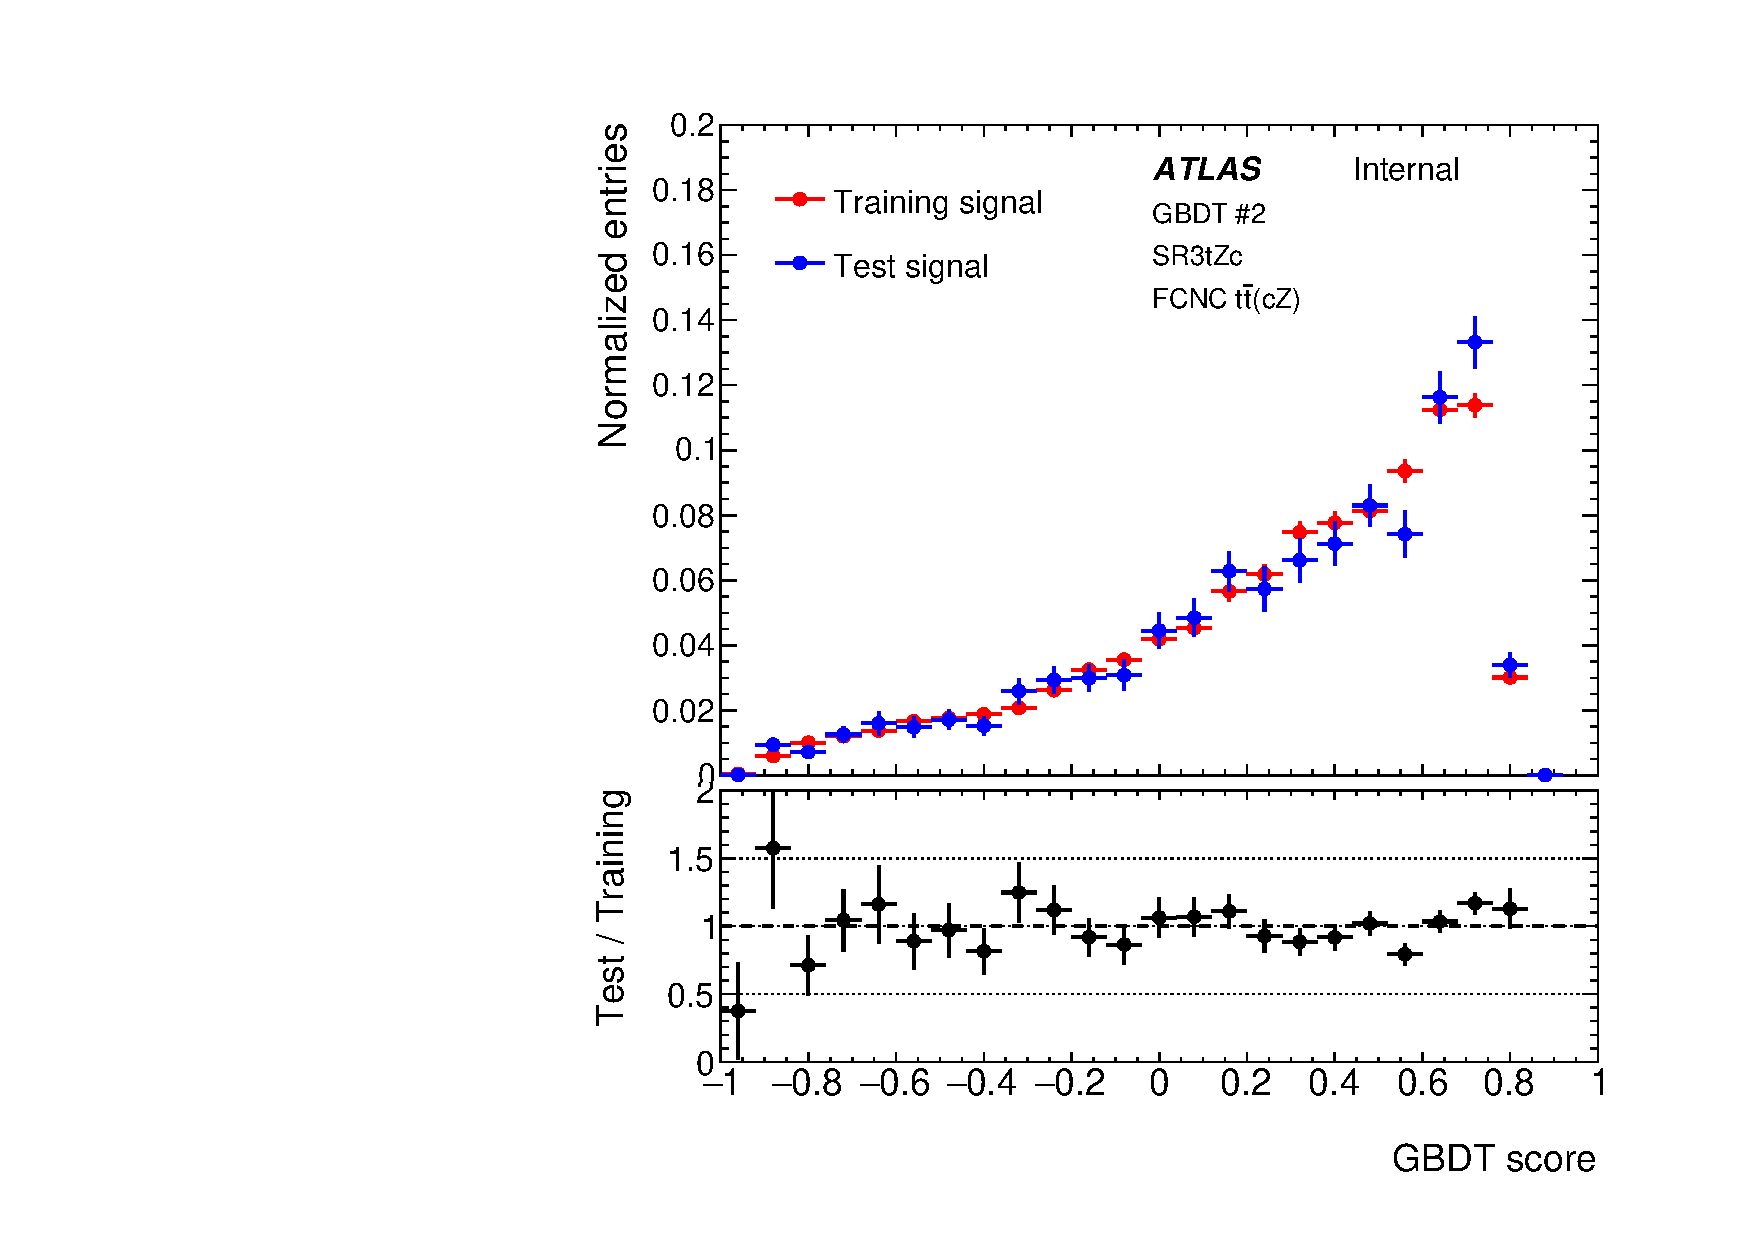
\includegraphics[width=.3\textwidth]{Chapters/CH6/figures/SR3_UsingSMT/BDT/GBDT_signal_Fold2} &
		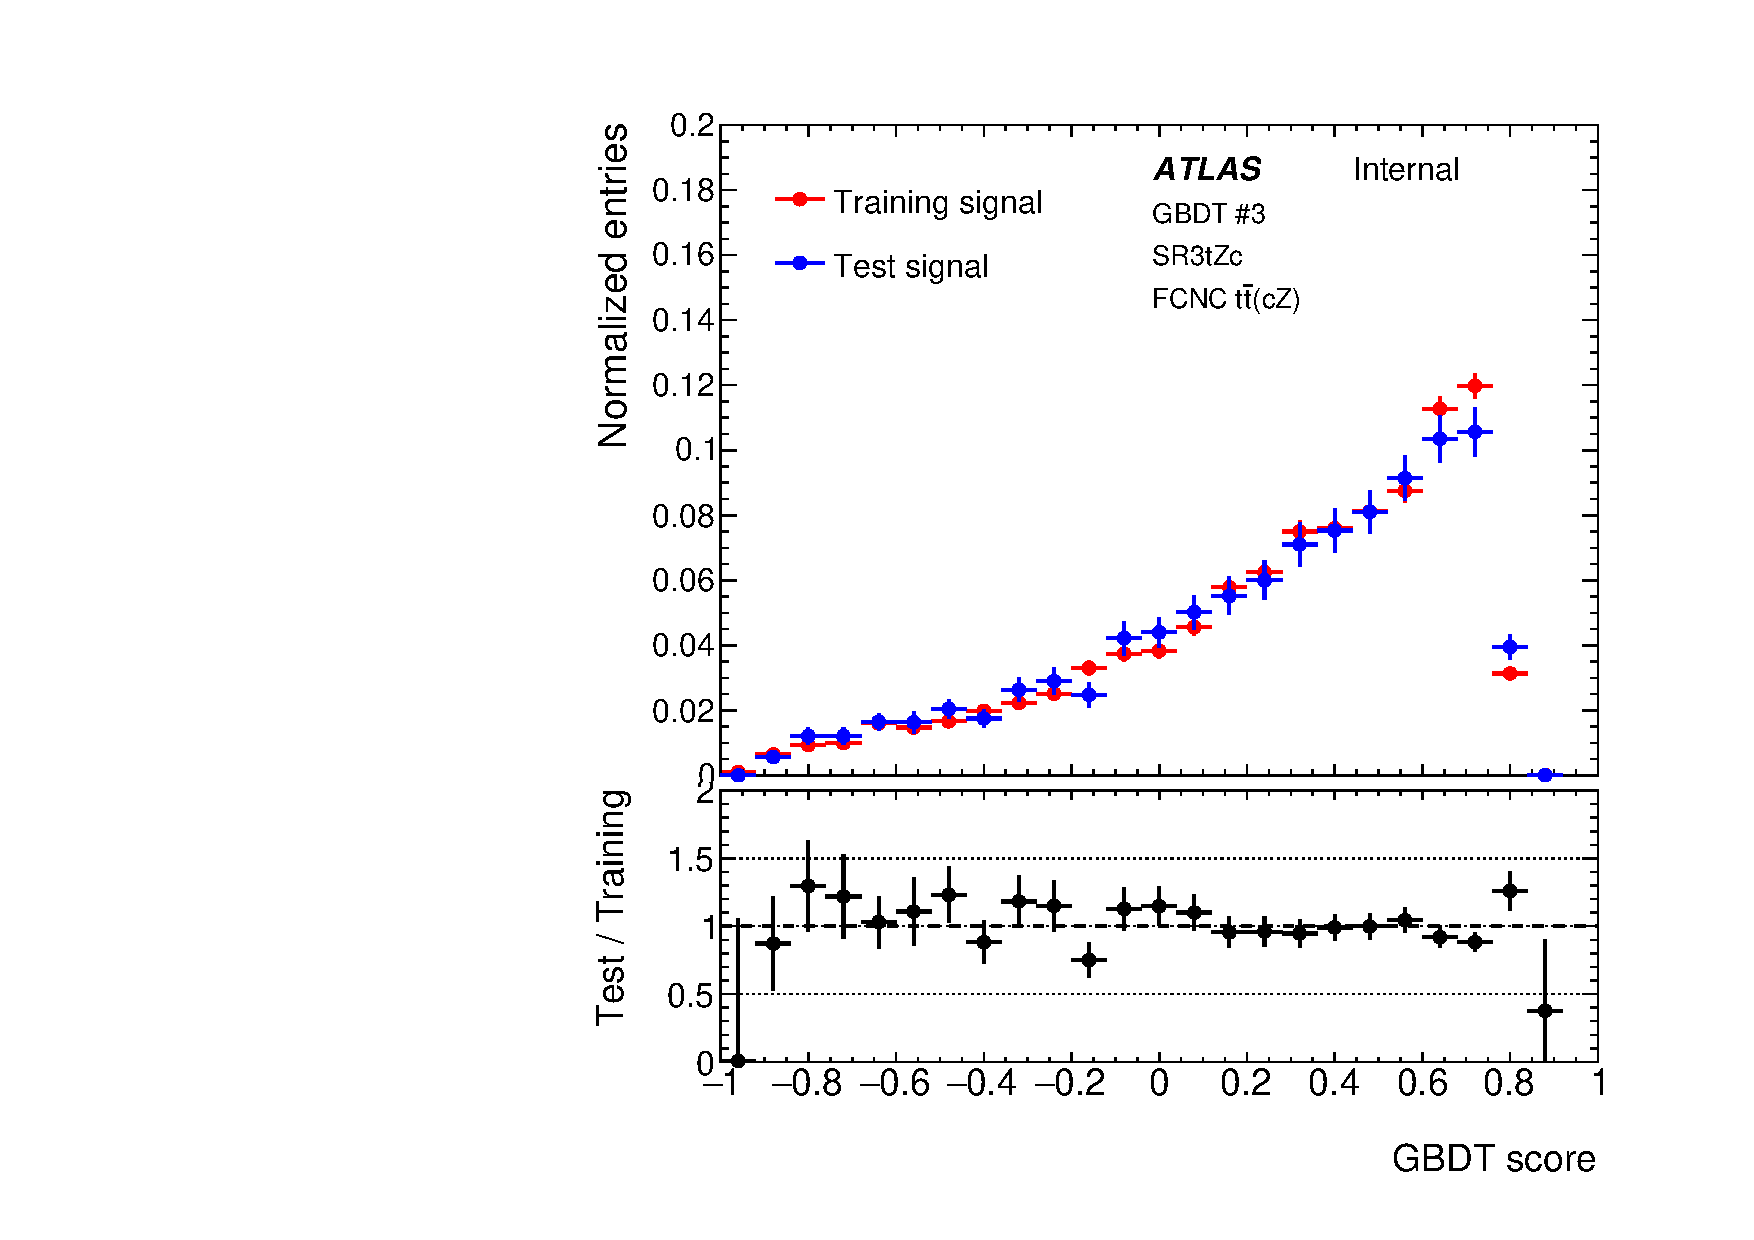
\includegraphics[width=.3\textwidth]{Chapters/CH6/figures/SR3_UsingSMT/BDT/GBDT_signal_Fold3} \\
		\multicolumn{3}{c}{
			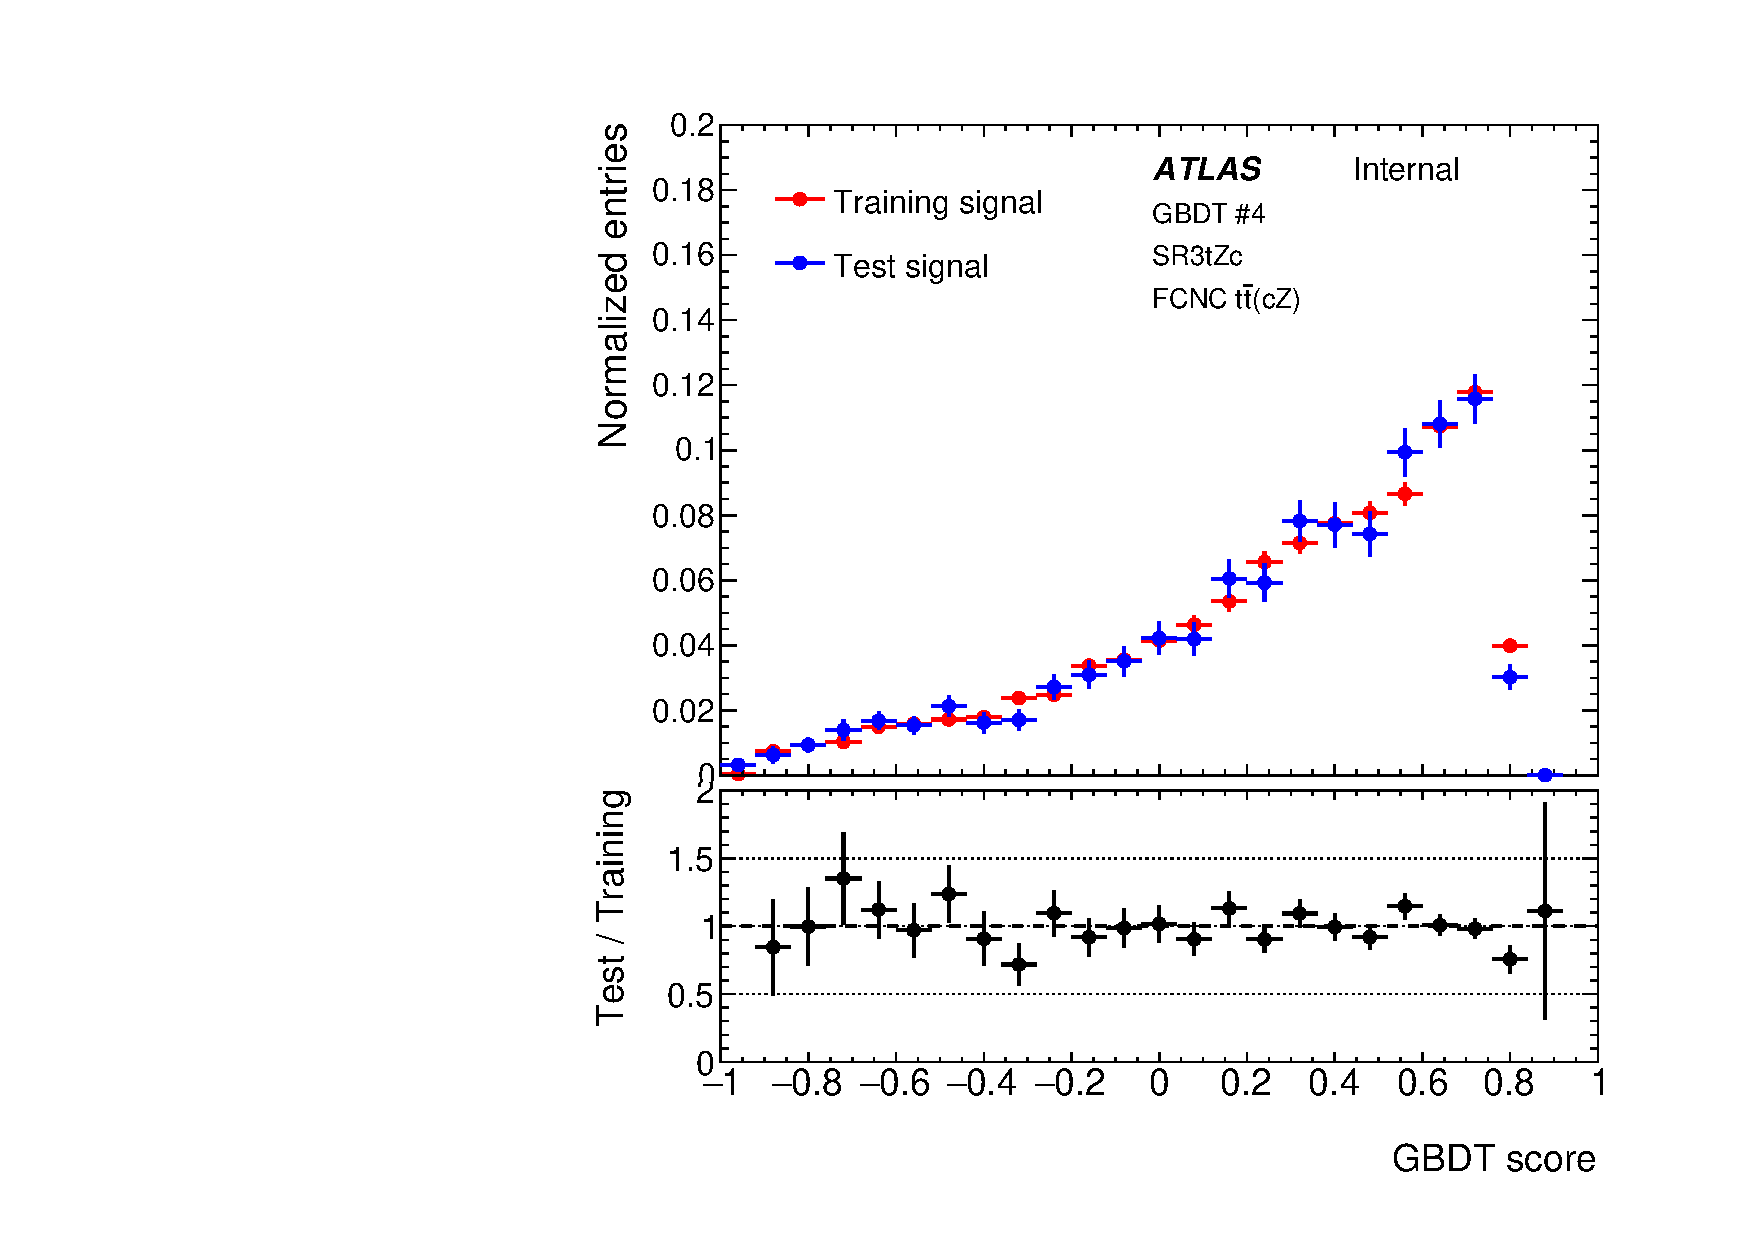
\includegraphics[width=.3\textwidth]{Chapters/CH6/figures/SR3_UsingSMT/BDT/GBDT_signal_Fold4}
			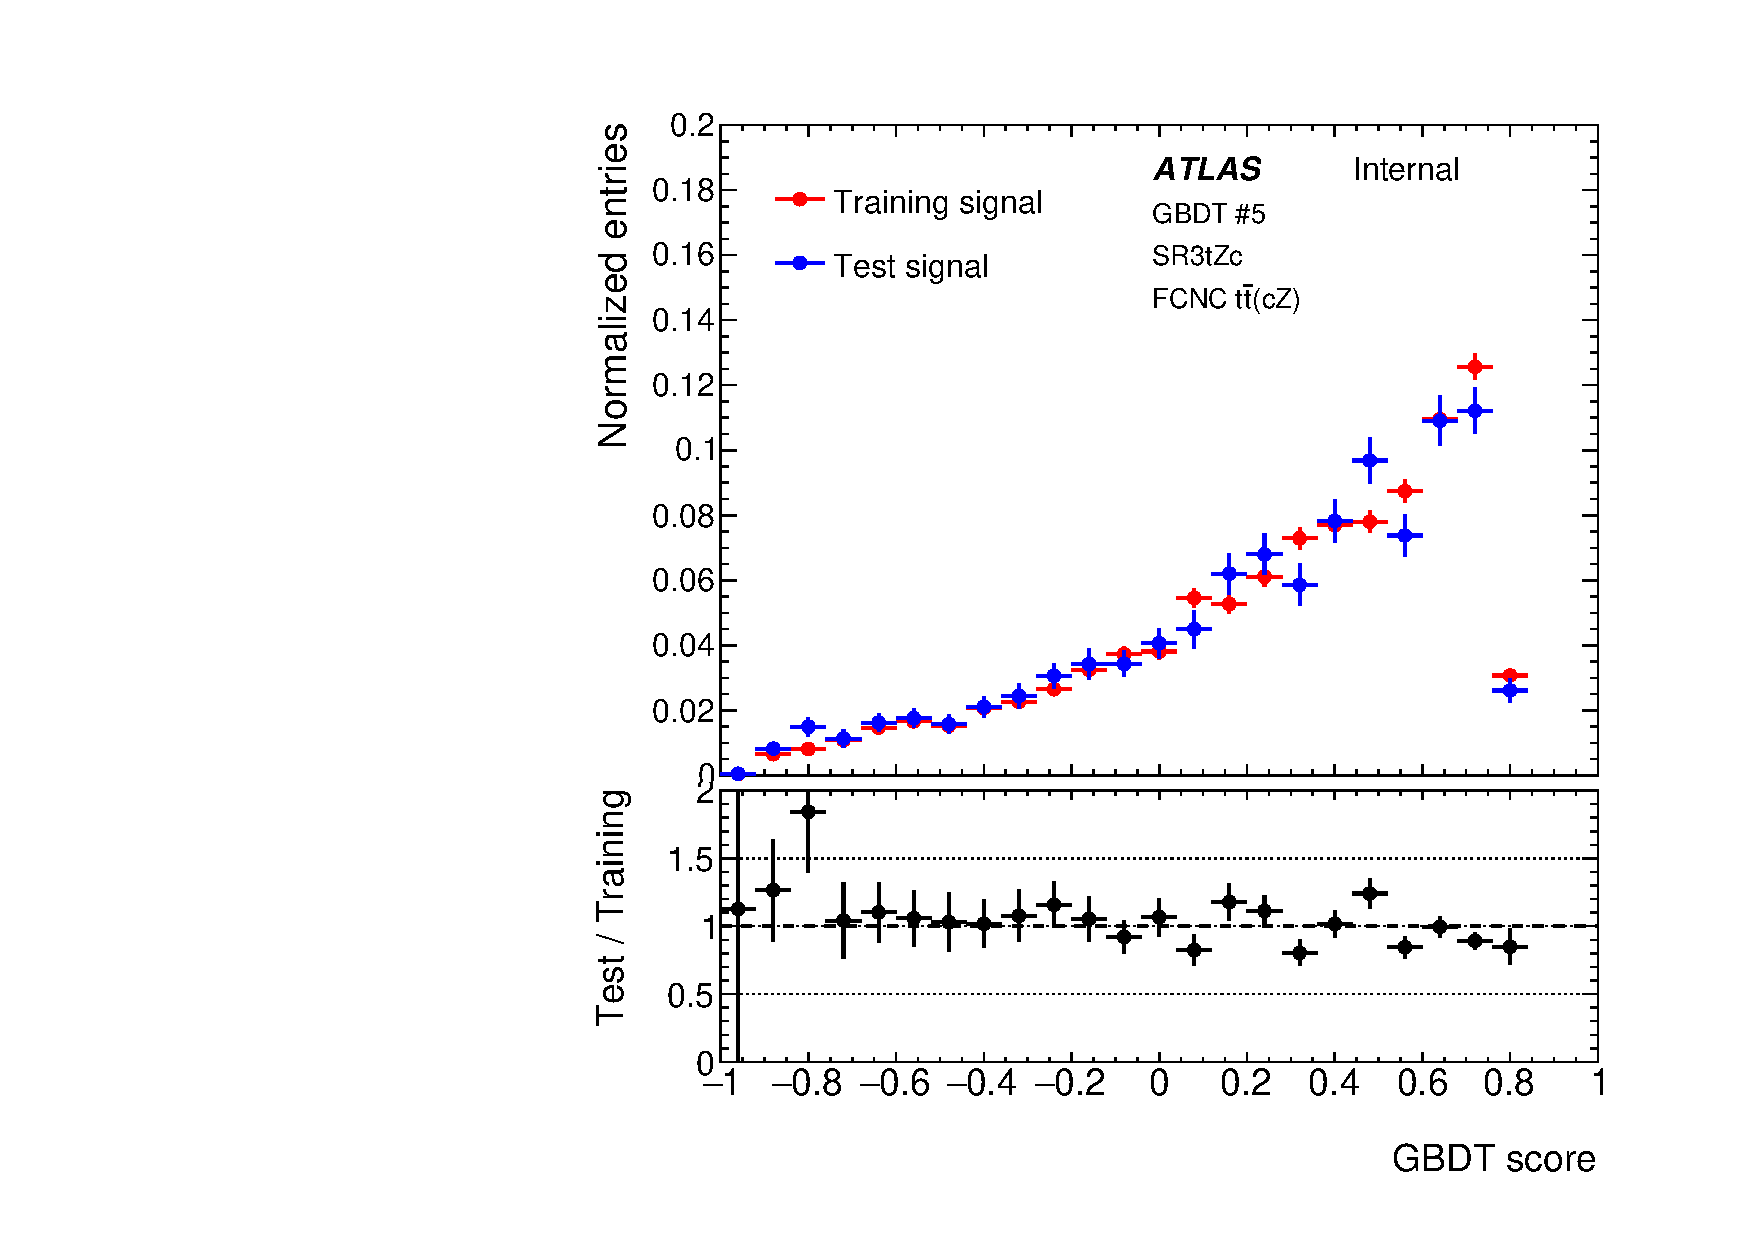
\includegraphics[width=.3\textwidth]{Chapters/CH6/figures/SR3_UsingSMT/BDT/GBDT_signal_Fold5}} \\
	\end{tabular}
	\caption{ The FCNC \ttbar decay signal GBDT output score distribution for each of five GBDTs trained in SR3 for the \Dthree discriminant.
		Final set of input variables is used in the training.
		Comparing results between training and test samples.
	}%
	\label{app:BDT:fig:SR3:GBDTsigFinalSet}
\end{figure}

\begin{figure}[!htbp]
	\centering
	\begin{tabular}{ccc}
		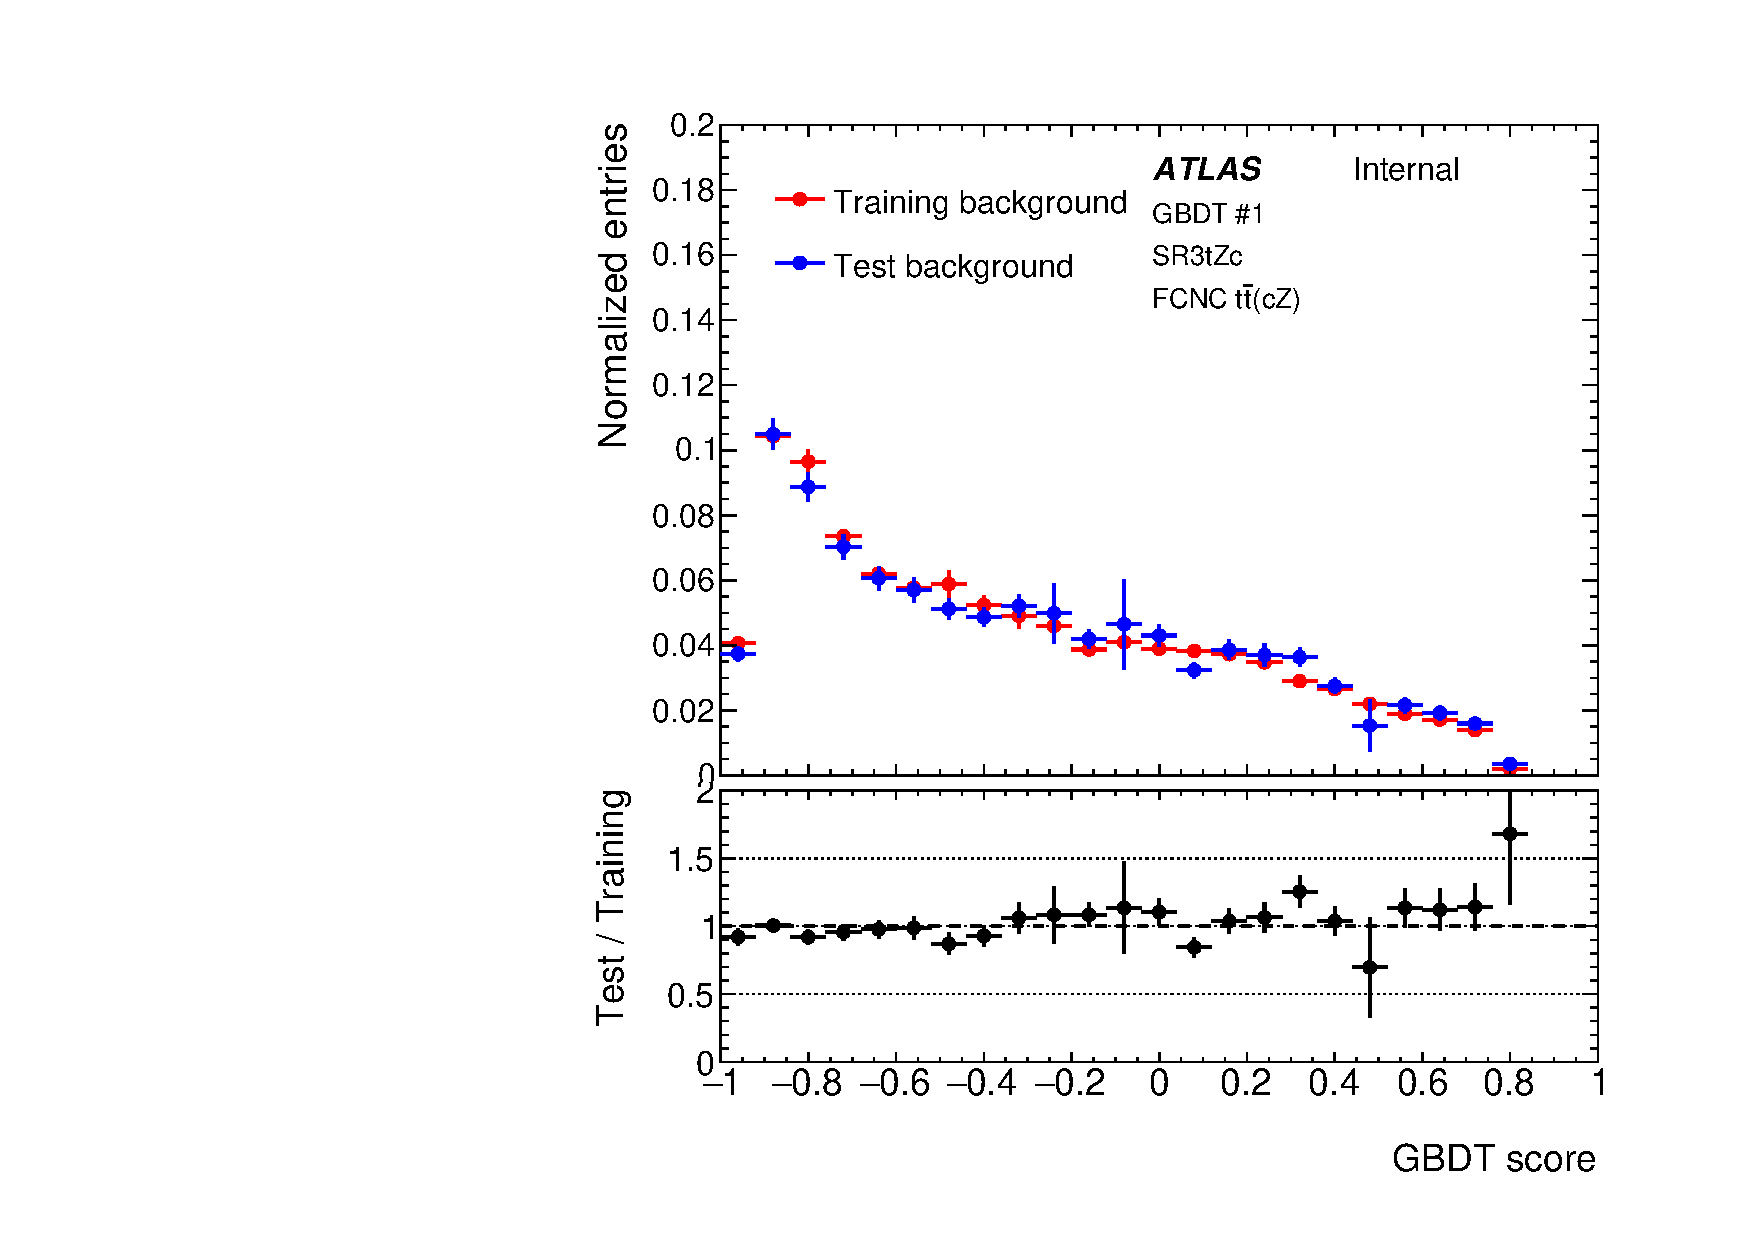
\includegraphics[width=.295\textwidth]{Chapters/CH6/figures/SR3_UsingSMT/BDT/GBDT_background_Fold1} &
		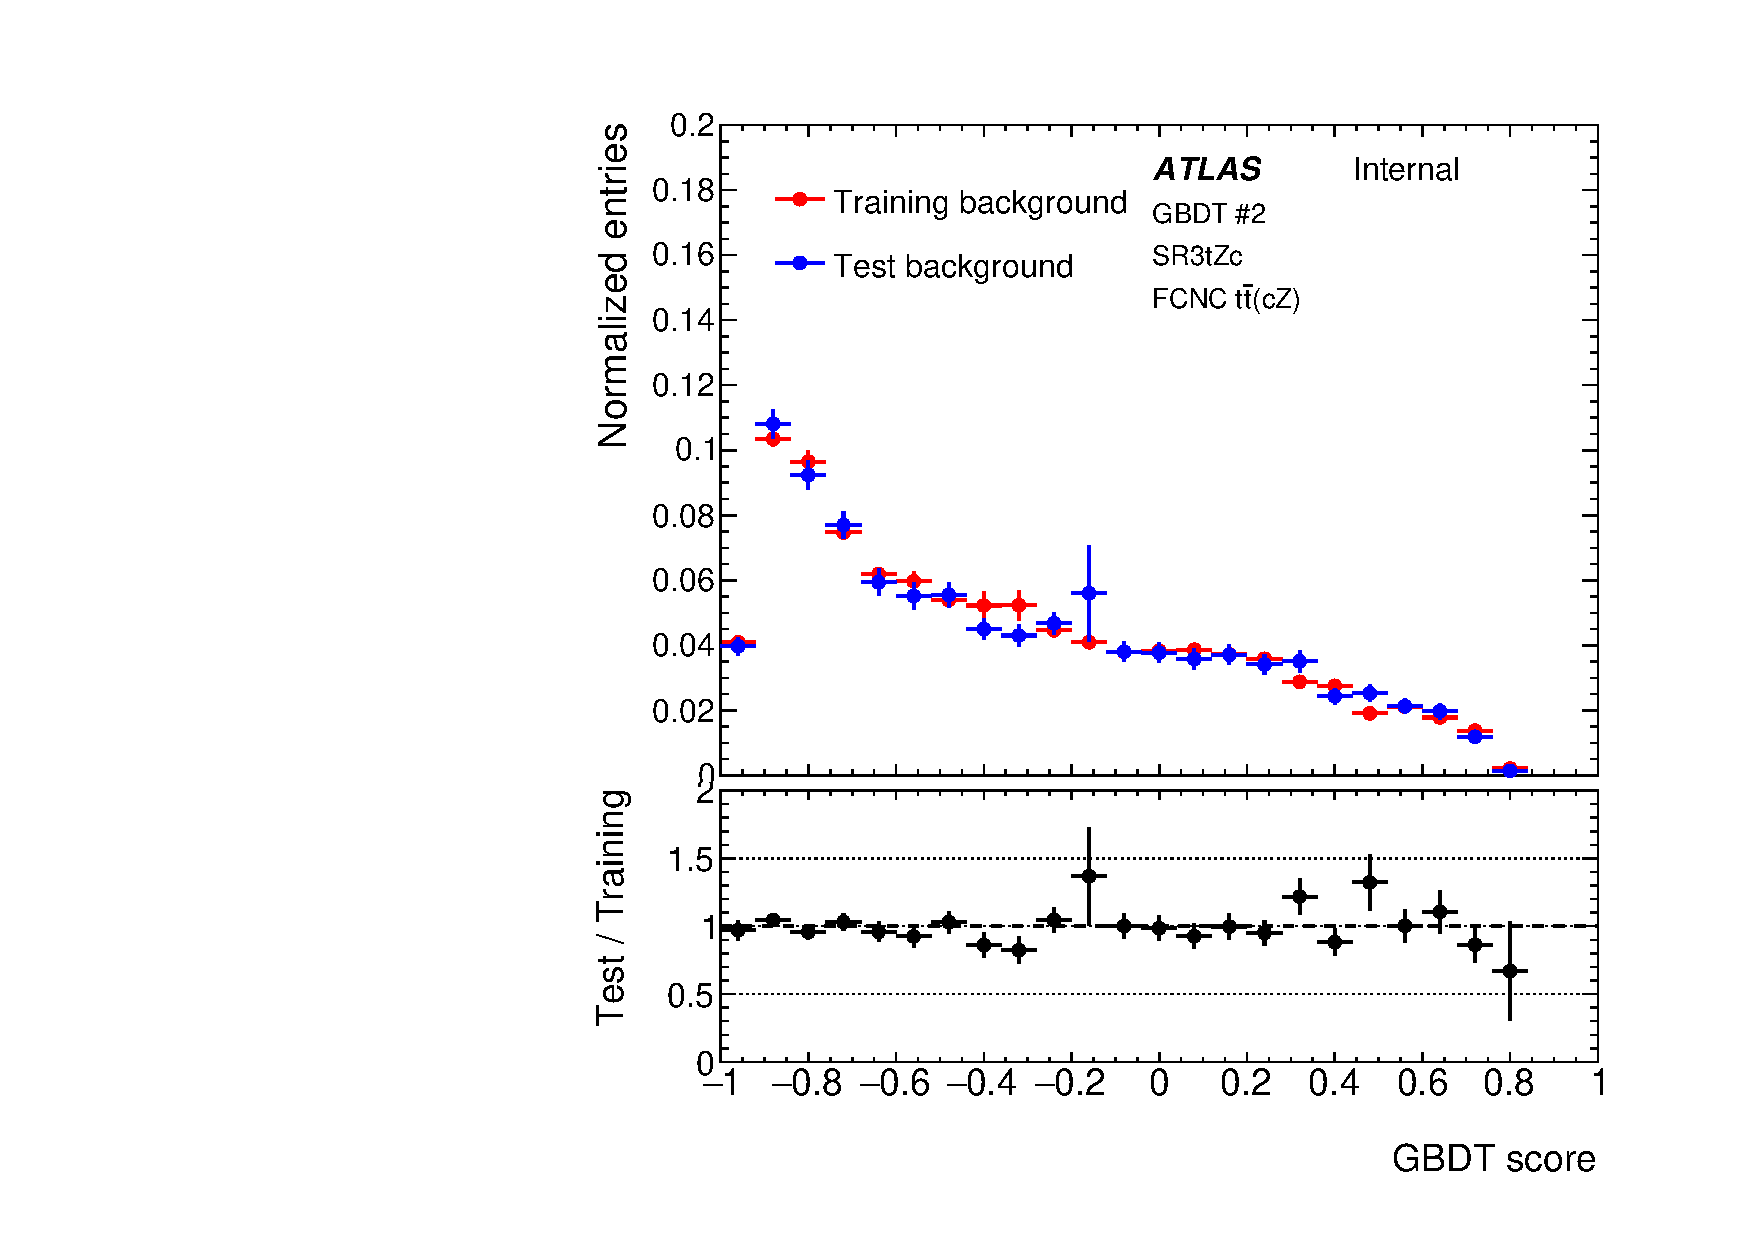
\includegraphics[width=.295\textwidth]{Chapters/CH6/figures/SR3_UsingSMT/BDT/GBDT_background_Fold2} &
		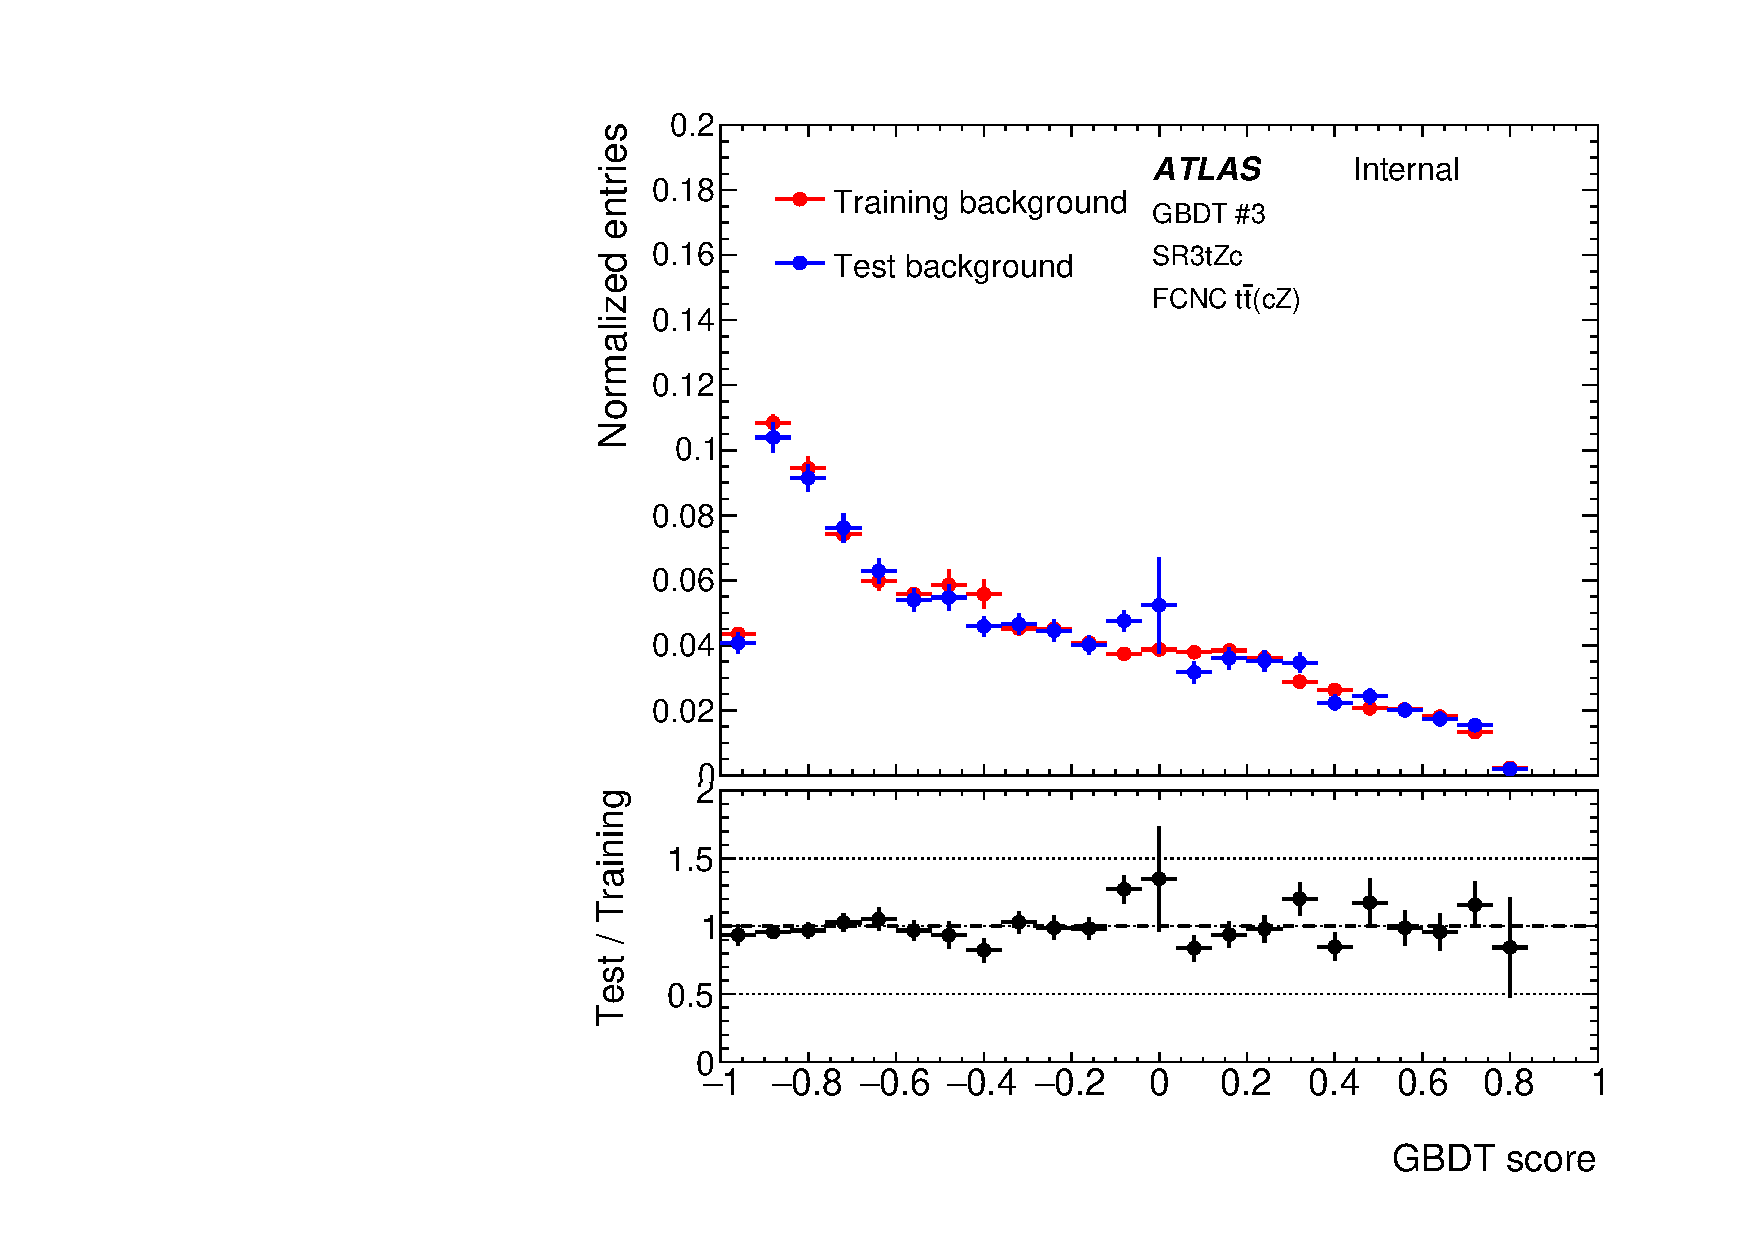
\includegraphics[width=.295\textwidth]{Chapters/CH6/figures/SR3_UsingSMT/BDT/GBDT_background_Fold3} \\
		\multicolumn{3}{c}{
		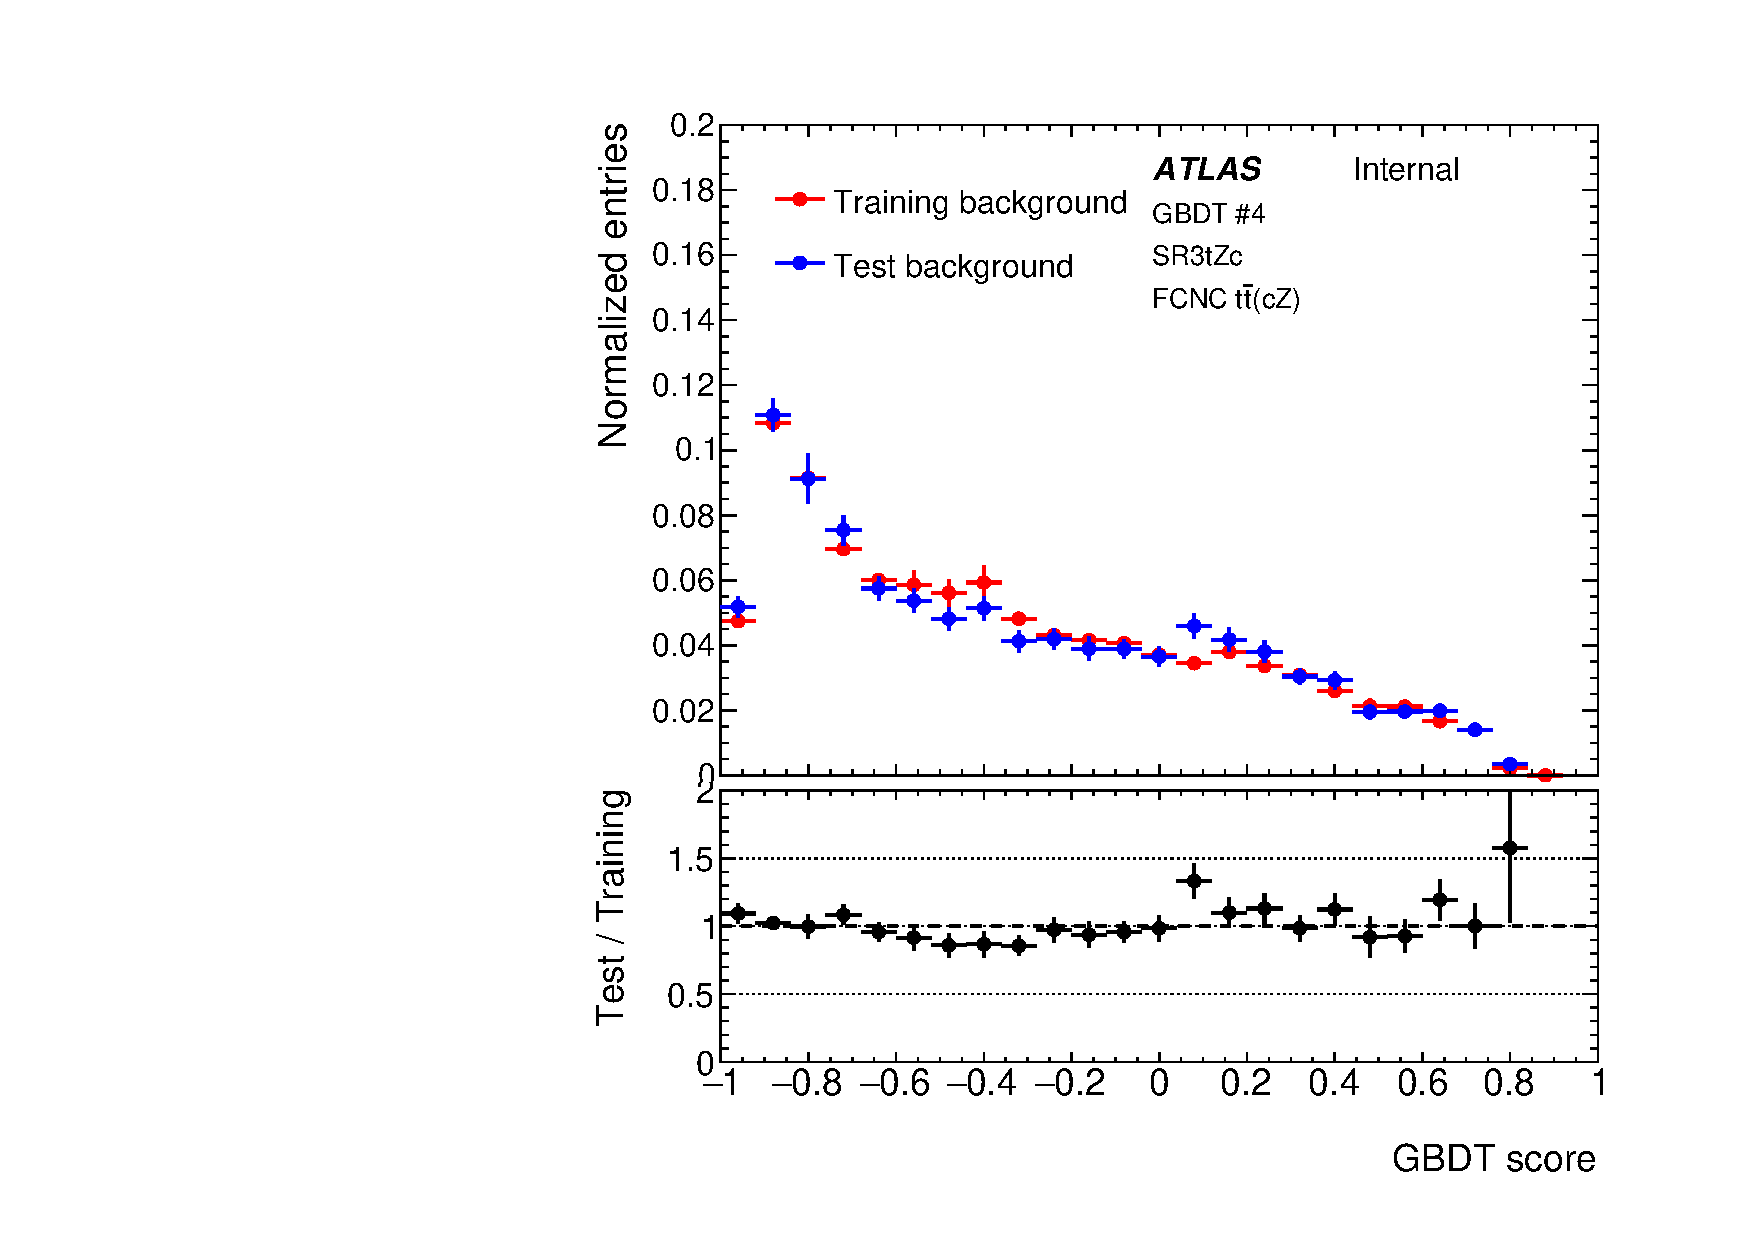
\includegraphics[width=.295\textwidth]{Chapters/CH6/figures/SR3_UsingSMT/BDT/GBDT_background_Fold4}
		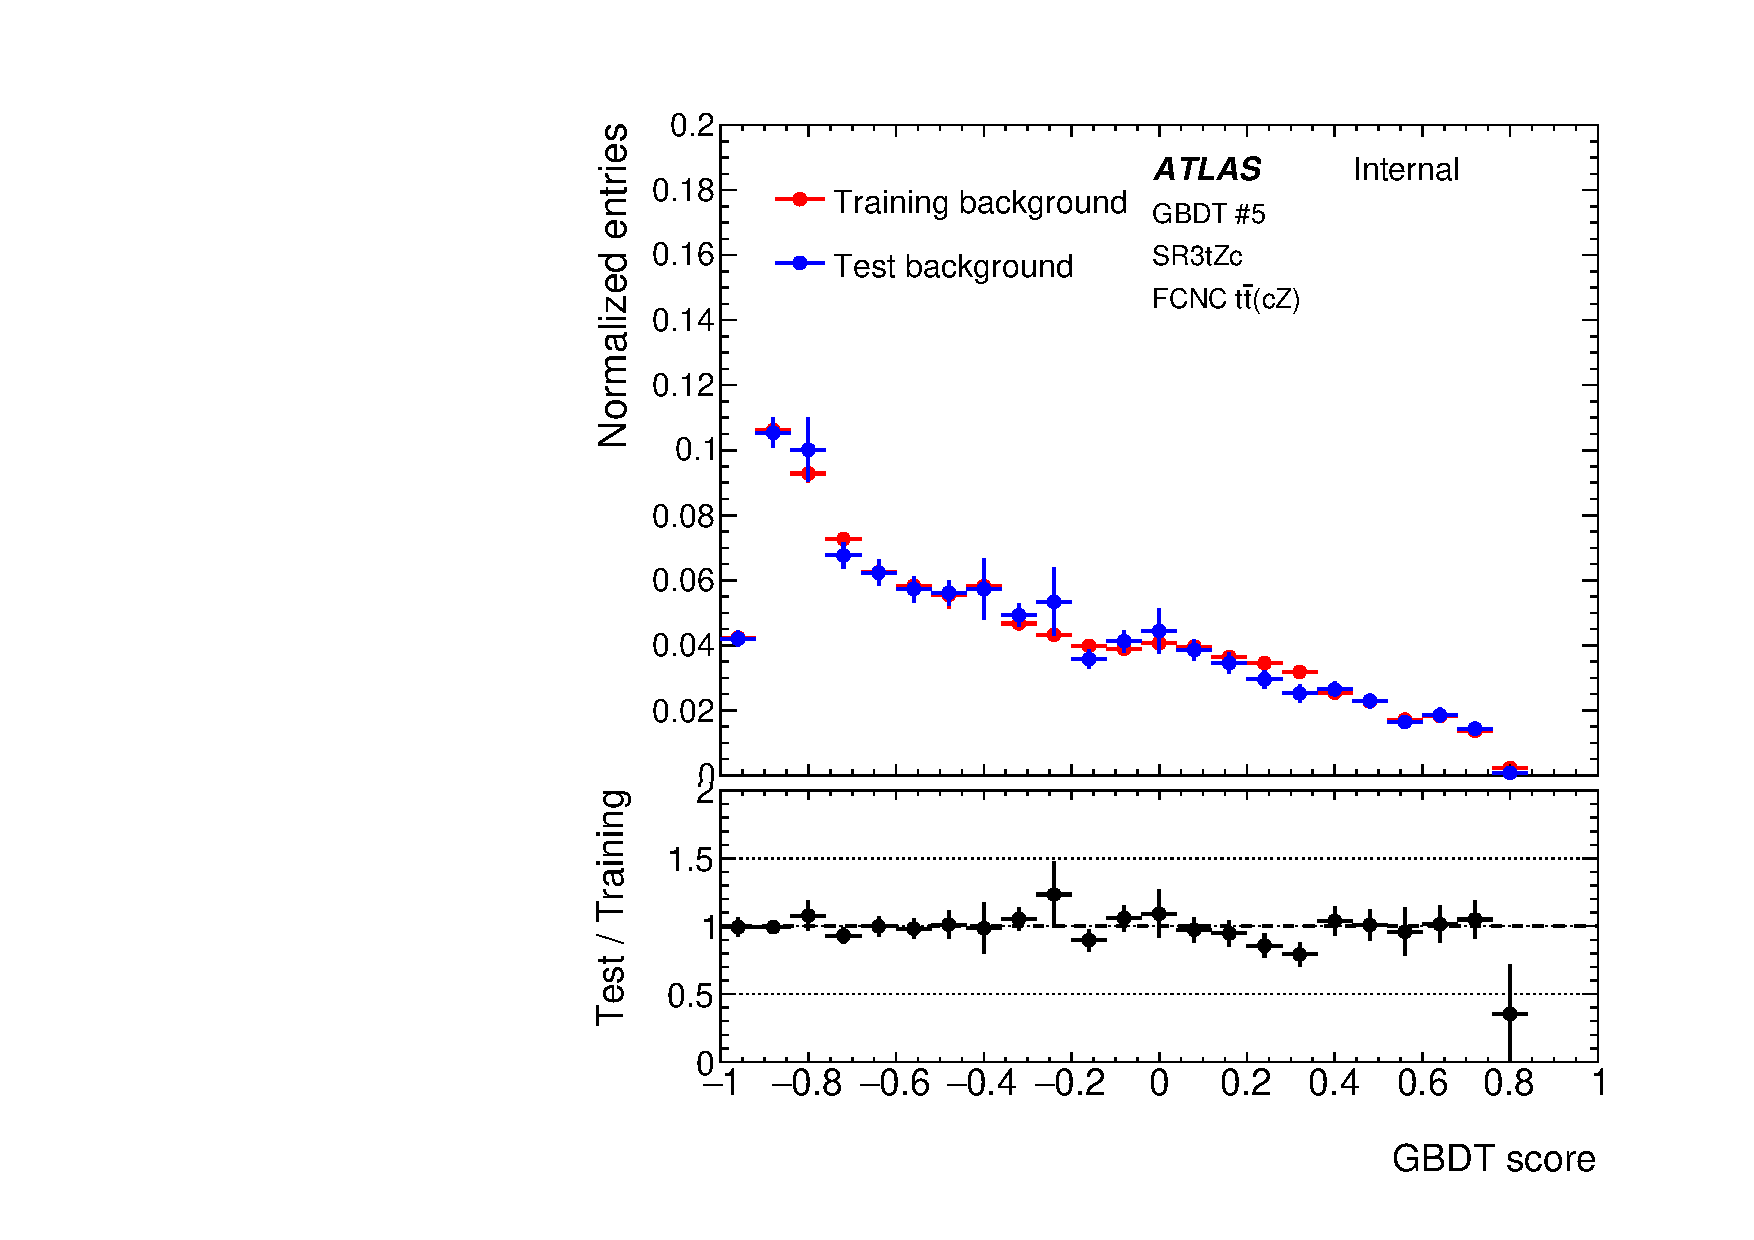
\includegraphics[width=.295\textwidth]{Chapters/CH6/figures/SR3_UsingSMT/BDT/GBDT_background_Fold5}} \\
	\end{tabular}
	\caption{ The background GBDT output score distribution for each of five GBDTs trained in SR3 for the \Dthree discriminant.
		Final set of input variables is used in the training.
		Comparing results between training and test samples.
	}%
	\label{app:BDT:fig:SR3:GBDTbkgFinalSet}
\end{figure}

\begin{figure}[!htbp]
	\centering
	\begin{tabular}{c}
		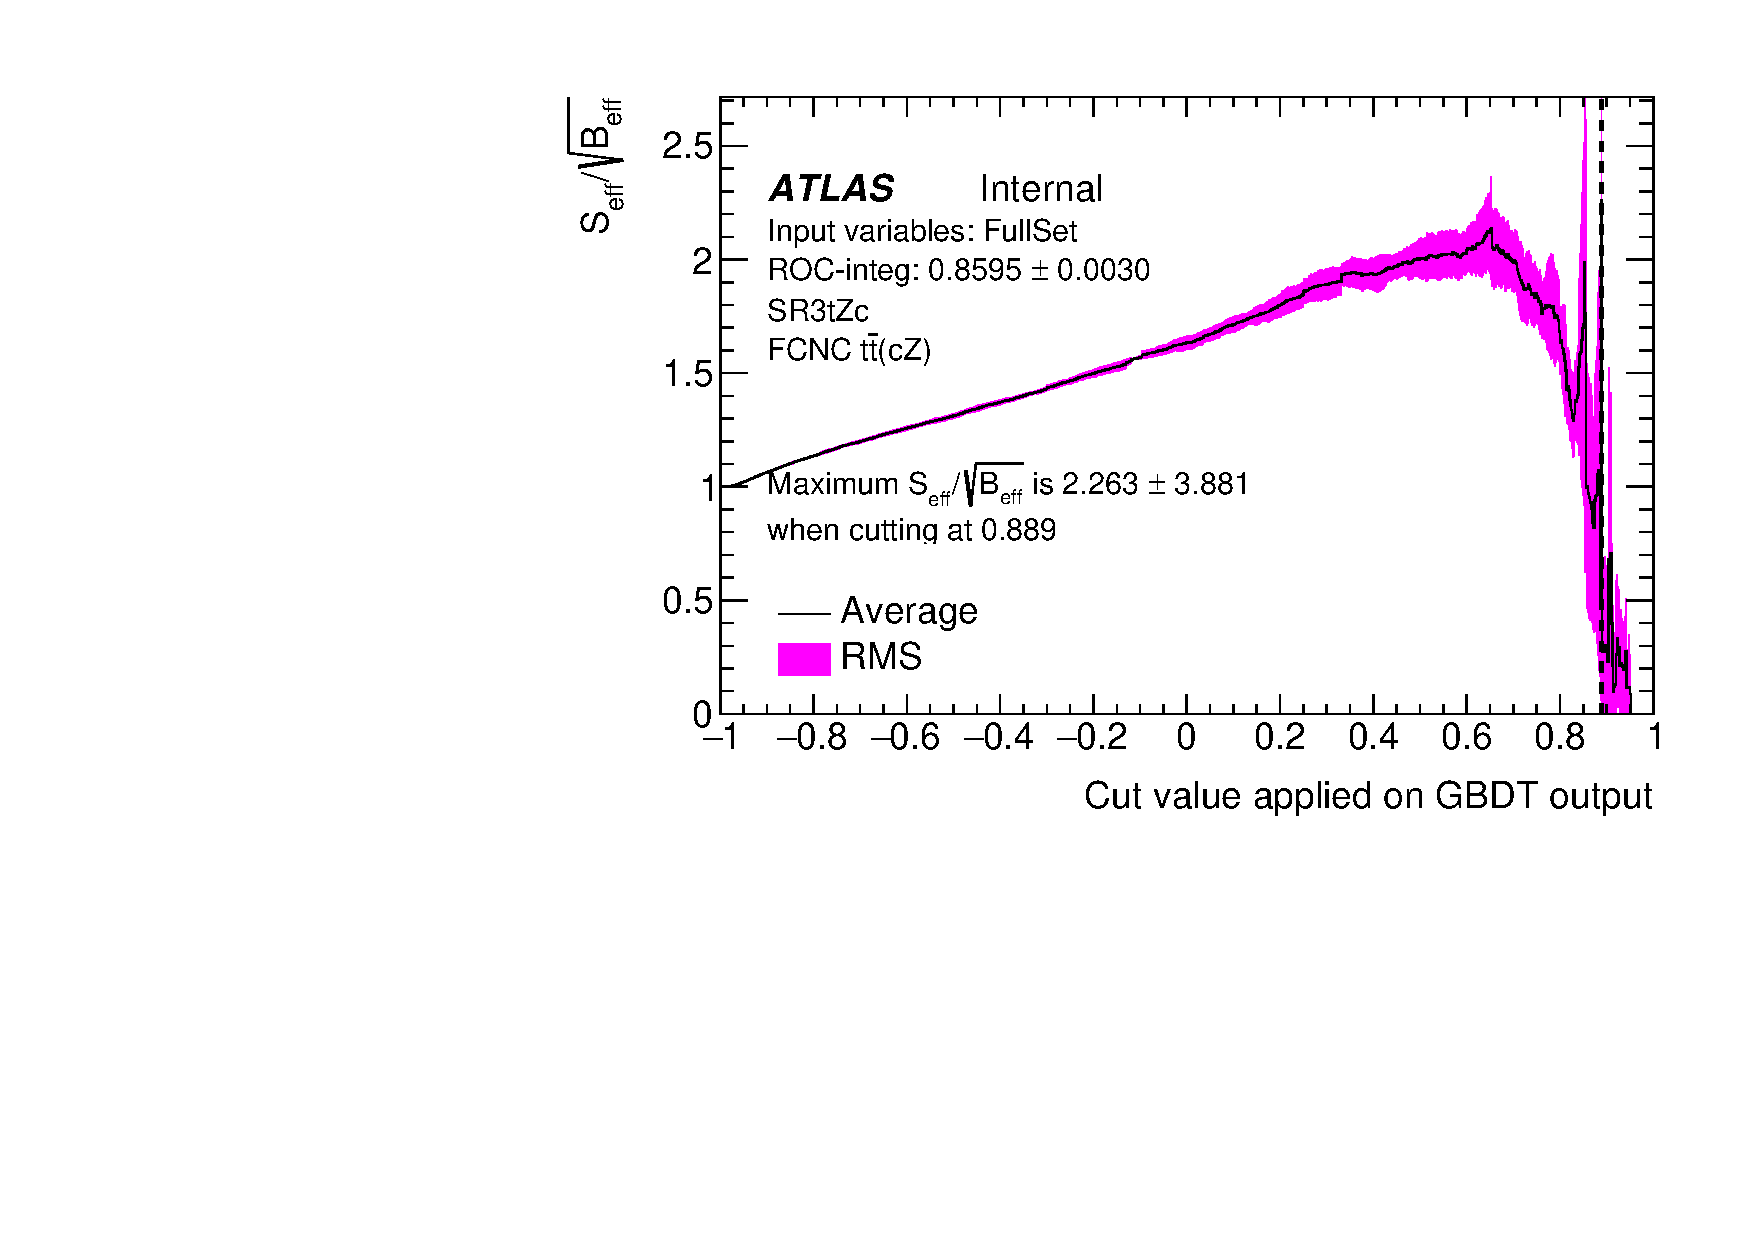
\includegraphics[width=.65\textwidth]{Chapters/CH6/figures/SR3_UsingSMT/BDT/FullSet/CutEff_FullSet}\\
		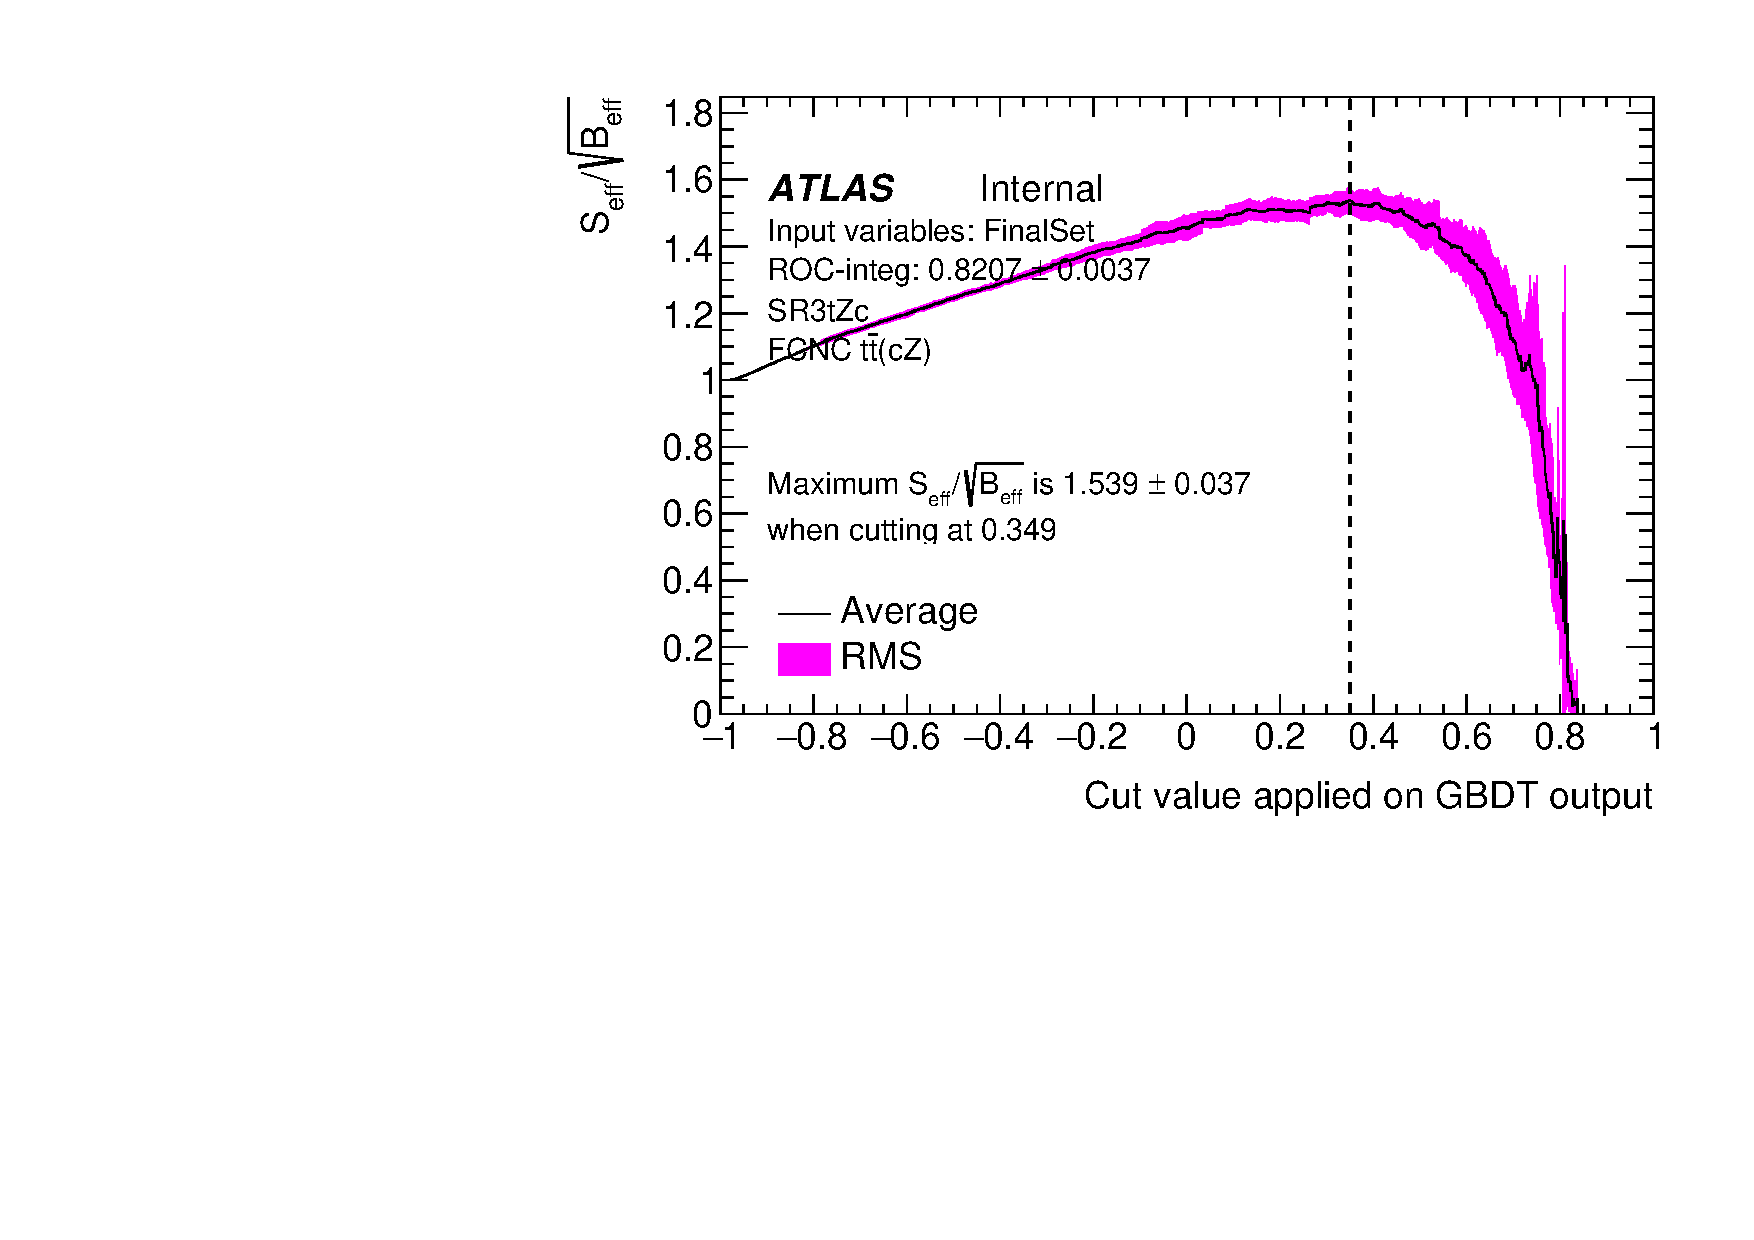
\includegraphics[width=.65\textwidth]{Chapters/CH6/figures/SR3_UsingSMT/BDT/FinalSet/CutEff_FinalSet}
	\end{tabular}
	\caption{ The $S_{\text{eff}}/\sqrt{B_{\text{eff}}}$ value averaged over the validation folds as a function of the cut on the BDT output score with full set (up) and final set (down) of input variables in the SR3.}
%	Values are calculated only if $S_{\text{eff}}$ and $B_{\text{eff}}$ are above 1\% to avoid statistically unstable results.}
	\label{app:BDT:fig:SR3:CutEff}
\end{figure}

\section{Hyper-parameters optimisation}
Once the final set of input variables are defined, the BDT hyper-parameters optimisation is performed.
The following BDT paremeters~\cite{TMVA} and values are considered with total of 144 combination:
NTrees=[400,600,800,1000], minNodSize=[2.0,4.0,6.0], shrinkage=[0.025,0.05,0.1], maxDepth=[1,2,3,4].
~\Cref{app:BDT:fig:SR3:HPO} presents the maximum value of $S_{\text{eff}}/\sqrt{B_{\text{eff}}}$ by cutting the BDT output score, and the ROC integral,
averaged over the validation folds, as a function of BDT hyper-parameters combination.\\
The difference between highest and lowest values of ROC integral
with the different BDT hyper-parameters combinations is $\sim2\%$.
These result indicate that the BDT performance is stable and not much can be improved with the hyper-parameters.\\
The average ROC integral (0.8207 with RMS of 0.0037) obtained with the reference BDT parameters (see~\cref{app:BDT:tab:param}) is almost identical to the highest value of ROC integral (0.8255 with RMS of 0.0028) obtained from the hyper-parameters optimisation.

\begin{figure}[!htbp]
	\centering
	\begin{tabular}{c}
		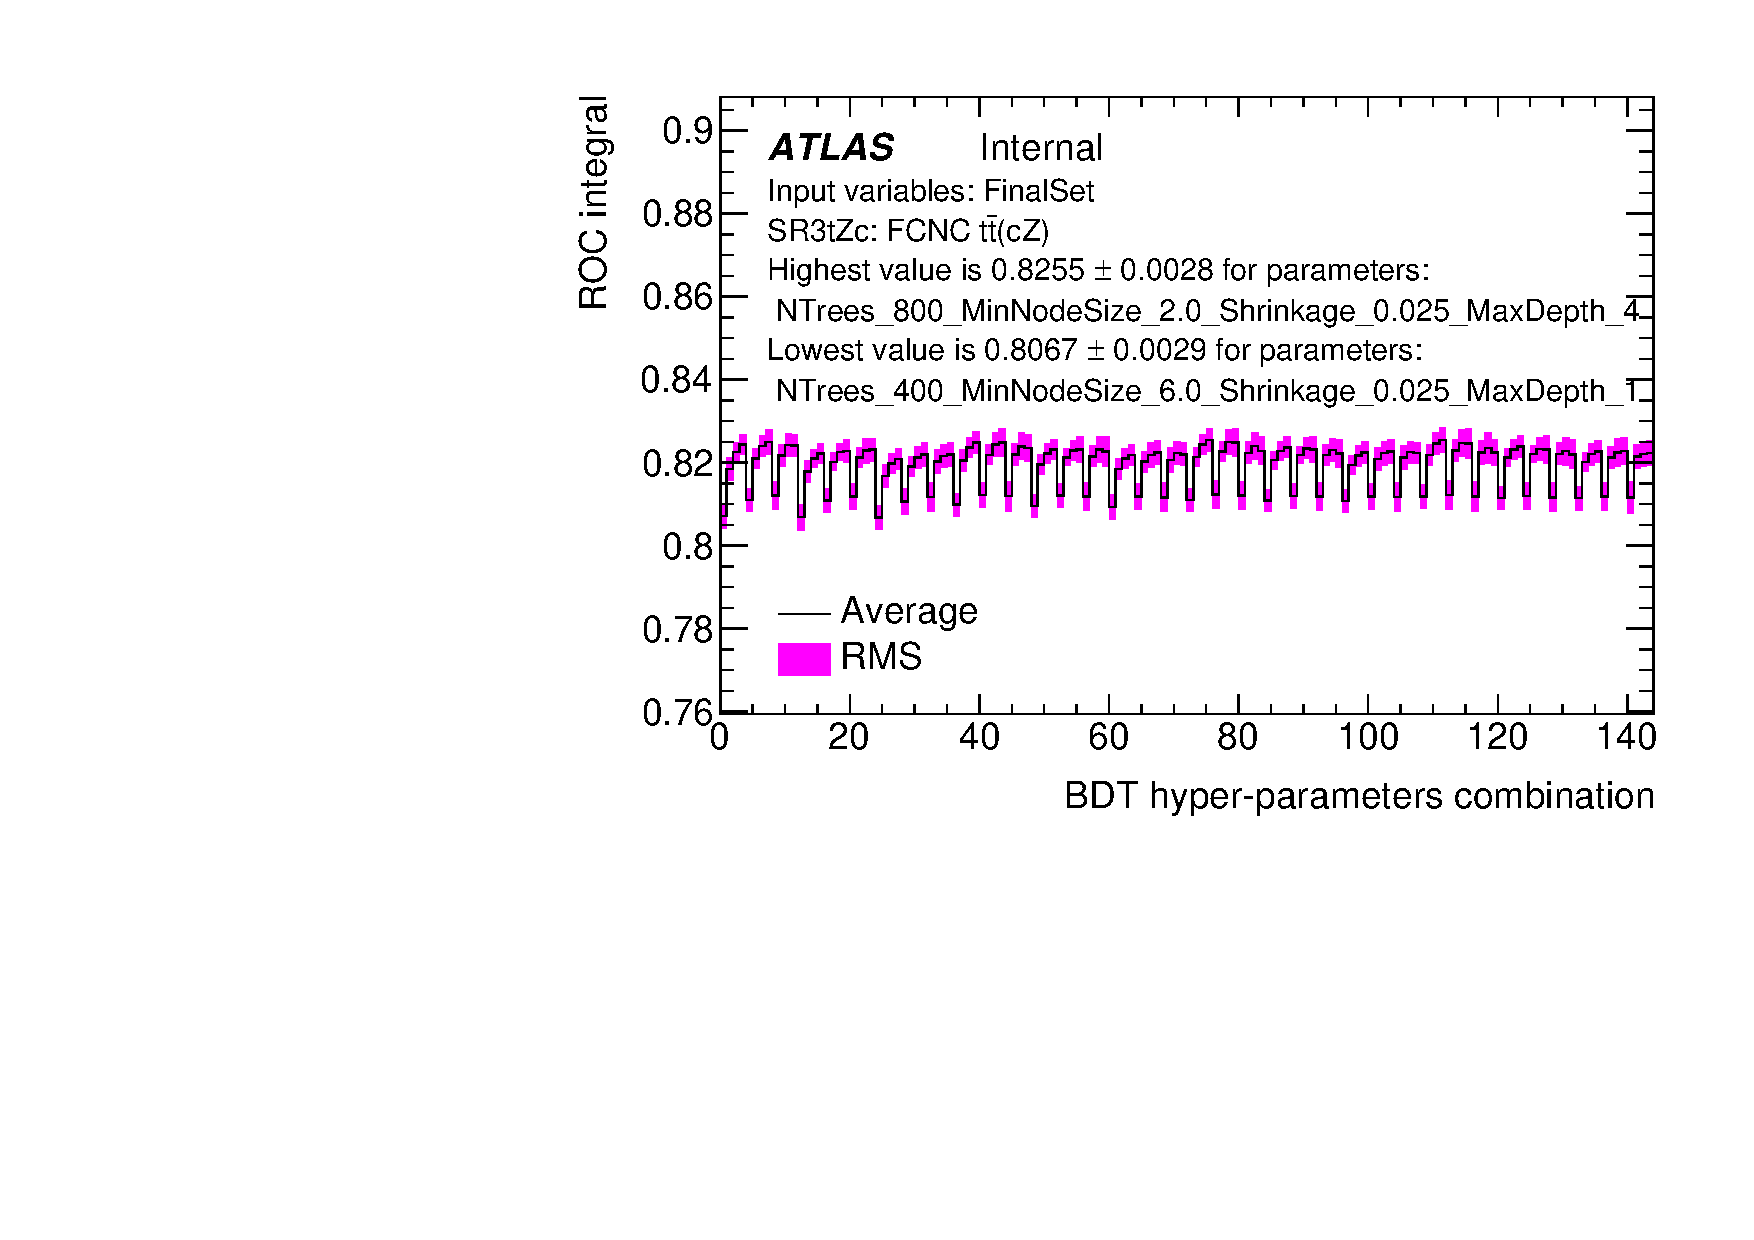
\includegraphics[width=.6\textwidth]{Chapters/CH6/figures/SR3_UsingSMT/BDT/FinalSet/HPO/ROC_integral}
	\end{tabular}
	\caption{ROC integral, averaged over the validation folds,
		as a function of BDT hyper-parameters combination in the SR3. The highest and lowest values of $S_{\text{eff}}/\sqrt{B_{\text{eff}}}$ and ROC integral are presented on the plots as well as
		the corresponding BDT parameters values.}
	\label{app:BDT:fig:SR3:HPO}
\end{figure}


%\end{verse}
%\end{samepage}
%\begin{figure}[htbp]
%	\centering
%	\begin{tabular}{ccc}
%		\includegraphics[width=.32\textwidth]{Chapters/CH6/figures/SR3_UsingSMT/BDT/FinalSet/HPO/{ROC_FinalSet_Fold1_NTrees_800_MinNodeSize_2.0_Shrinkage_0.05_MaxDepth_2}.pdf} &
%		\includegraphics[width=.32\textwidth]{Chapters/CH6/figures/SR3_UsingSMT/BDT/FinalSet/HPO/{ROC_FinalSet_Fold2_NTrees_800_MinNodeSize_2.0_Shrinkage_0.05_MaxDepth_2}.pdf} &
%		\includegraphics[width=.32\textwidth]{Chapters/CH6/figures/SR3_UsingSMT/BDT/FinalSet/HPO/{ROC_FinalSet_Fold3_NTrees_800_MinNodeSize_2.0_Shrinkage_0.05_MaxDepth_2}.pdf} \\
%		\multicolumn{3}{c}{
%			\includegraphics[width=.32\textwidth]{Chapters/CH6/figures/SR3_UsingSMT/BDT/FinalSet/HPO/{ROC_FinalSet_Fold4_NTrees_800_MinNodeSize_2.0_Shrinkage_0.05_MaxDepth_2}.pdf}
%			\includegraphics[width=.32\textwidth]{Chapters/CH6/figures/SR3_UsingSMT/BDT/FinalSet/HPO/{ROC_FinalSet_Fold5_NTrees_800_MinNodeSize_2.0_Shrinkage_0.05_MaxDepth_2}.pdf}} \\
%	\end{tabular}
%	\caption{ The ROC curves obtained with the reference BDT parameters (see~\cref{app:BDT:tab:param}) in the SR3 for each of five folds.
%		Final set of input variables is used in the training. Comparing results between training and test samples.
%	}%
%	\label{app:BDT:fig:SR3:RefParamROC}
%\end{figure}
%
%\begin{figure}[htbp]
%	\centering
%	\begin{tabular}{ccc}
%		\includegraphics[width=.32\textwidth]{Chapters/CH6/figures/SR3_UsingSMT/BDT/FinalSet/HPO/{ROC_FinalSet_Fold1_NTrees_1000_MinNodeSize_2.0_Shrinkage_0.025_MaxDepth_4}.pdf} &
%		\includegraphics[width=.32\textwidth]{Chapters/CH6/figures/SR3_UsingSMT/BDT/FinalSet/HPO/{ROC_FinalSet_Fold2_NTrees_1000_MinNodeSize_2.0_Shrinkage_0.025_MaxDepth_4}.pdf} &
%		\includegraphics[width=.32\textwidth]{Chapters/CH6/figures/SR3_UsingSMT/BDT/FinalSet/HPO/{ROC_FinalSet_Fold3_NTrees_1000_MinNodeSize_2.0_Shrinkage_0.025_MaxDepth_4}.pdf} \\
%		\multicolumn{3}{c}{
%			\includegraphics[width=.32\textwidth]{Chapters/CH6/figures/SR3_UsingSMT/BDT/FinalSet/HPO/{ROC_FinalSet_Fold4_NTrees_1000_MinNodeSize_2.0_Shrinkage_0.025_MaxDepth_4}.pdf}
%			\includegraphics[width=.32\textwidth]{Chapters/CH6/figures/SR3_UsingSMT/BDT/FinalSet/HPO/{ROC_FinalSet_Fold5_NTrees_1000_MinNodeSize_2.0_Shrinkage_0.025_MaxDepth_4}.pdf}} \\
%	\end{tabular}
%	\caption{ The ROC curves obtained with the BDT hyper-parameters giving the highest ROC-integral in the SR3 for each of five folds.
%		Final set of input variables is used in the training. Comparing results between training and test samples.
%	}%
%	\label{app:BDT:fig:SR3:HighestROC}
%\end{figure}

